Pipelines are critical for safe and efficient transportation of fluids across long distances.  For example, pipelines are used by utility companies to transport clean water and natural gas to homes for heating and living purposes.  Furthermore, pipelines are also used in agriculture to transport irrigation water to hydrate crops.  Moreover, pipelines are used by energy companies for transporting energy-rich hydrocarbons to fuel the world's transportation and manufacturing needs. In the United States, over 70\% of petroleum products are shipped by pipeline.  In Canada, the number increases to 97\% \cite{pipeline_transport}.  The latest data in 2014 estimates that there are about 3,500,000 km of operational pipelines across 120 countries \cite{CIA_pipeline}. Due to the world's dependency on pipelines for transporting their basic needs, ensuring its reliability and efficiency has a global-scale impact.

Typical pipelines have hundreds of digital measurements per minute and are hard to analyze; however, machine learning methods benefit greatly from large amounts of data. Thus, an opportunity was discovered where machine learning methods will be applied to pipelines used to transport petroleum products. The objectives of this project were to leverage machine learning to identify anomalous pipeline behaviour, and to build a real time optimization tool to automate, normalize and enhance the pipeline operation.

In this chapter, a time-series neural network classifier will first be introduced to detect anomalous activity within any pipeline equipment.  Then, a real time optimization tool based on a linear model optimized using mixed integer linear program will be introduced.  Due to confidentiality agreements, all data presented here-forth will be normalized, and all parties of this project will remain anomalous.

\section{Process Introduction}
Two separate pipelines, Line 11 and Line RM06A, were analyzed.  Line 11 is a simplistic pipeline; data from line 11 were used to build an anomaly detection tool.  Line RM06A was more complex; therefore, a real time optimization (RTO) tool was build for this line.

\subsection{Line 11}
The schematic of line 11 is shown in Figure \ref{fig:08Line11}. For Line 11, the objective was to build an anomaly detection tool for unexpected shut downs of its pumps.  

\begin{figure}[h]
    \centering
    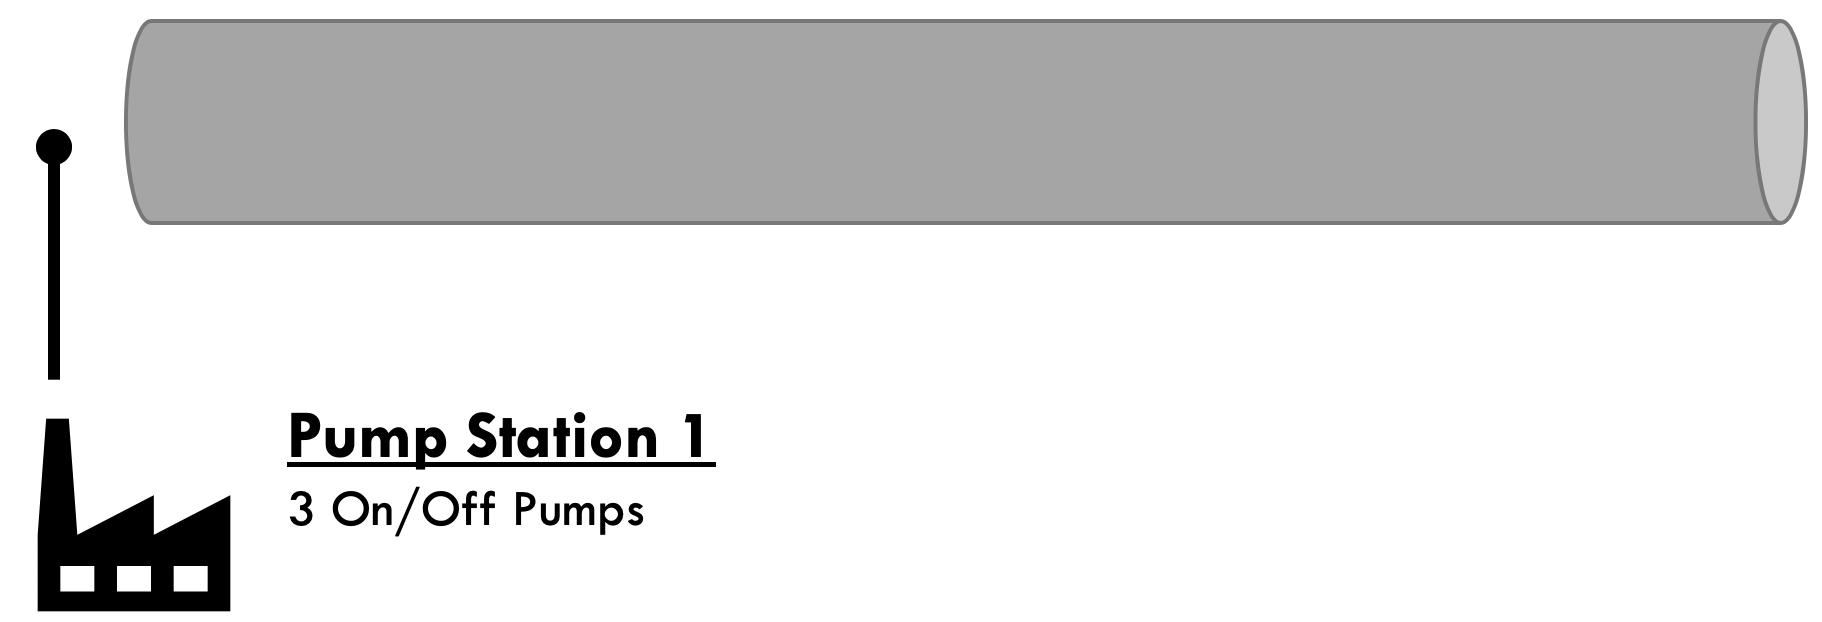
\includegraphics[scale=0.45]{images/08Line11.png}
    \caption{Schematic diagram of Line 11.}
    \label{fig:08Line11}
\end{figure}


\subsection{Line RM06A}
A schematic of line RM06A is shown in Figure \ref{fig:08RM06A}.  Line RM06A is a complex pipeline spanning 151 km and carries two products, a lighter sweet product and a heavier sour product. The two products are batched (i.e., rotate between sending each product) and each product is sent for approximately eight hours before switching to the other product. The American Petroleum Institute (API) gravity for the lighter and heavier products are roughly 40 and 20, respectively. For the rest of this chapter, the lighter and heavier product will be referred to as \textit{sweet crude} and \textit{sour crude}, respectively. The pipeline is operated between 1500 bbl/h to 3050 bbl/h for the majority of the time. 

\begin{figure}[h]
    \centering
    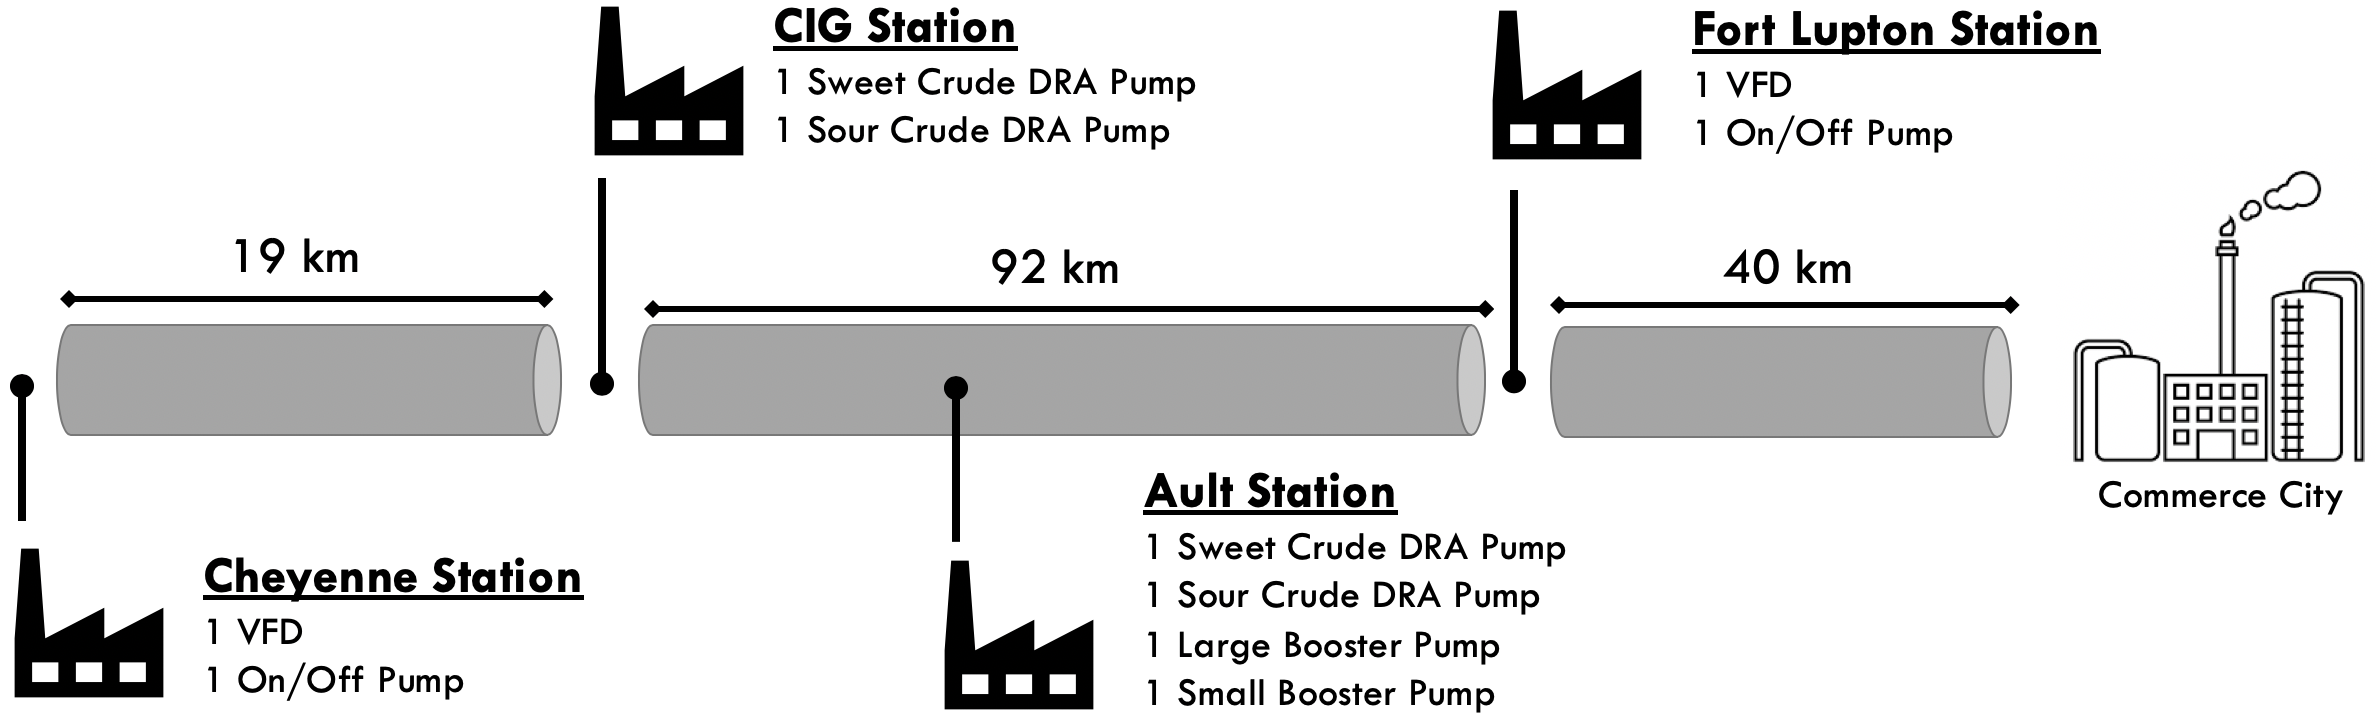
\includegraphics[scale=0.35]{images/08RM06A.png}
    \caption{Schematic diagram of Line RM06A.}
    \label{fig:08RM06A}
\end{figure}

Equipment wise, Line RM06A boasts eight pumps spread across four pump stations. Two pumps are variable frequency drives (VFD), while the rest are on/off pumps. Additionally, there are four drag reducing agent (DRA) injection pumps situated across the second and third pump stations. Each pump station contains a sour crude and sweet crude DRA pump. The sour and sweet crude uses different types of DRA.  The DRA is injected based on the product present at the pump station. 



\section{Anomaly Detection}
\subsection{Data Pre-processing}
\subsection{Data Set Creation}
\subsubsection{Generative Modelling}
\subsection{Model Identification}
\subsection{Conceptual Software Design}

\section{Real Time Optimization}
Modern control systems typically consists of three layers: real time optimization (RTO), supervisory control and regulatory control.  From the top, real time optimization is evaluated the least frequently, and performs a steady state optimization of the process.  The outputs of RTO are the ideal set points for all equipment.  Next, the supervisory control layer performs dynamic optimization to identify the most efficient input trajectory to achieve the set points from RTO. Supervisory control is evaluated faster than RTO, but slower than regulatory control. Model predictive control (MPC) and economic model predictive control (EMPC) are typical supervisory control frameworks. Finally, the regulatory controllers actuate physical equipment to achieve the input trajectory given by the supervisory control layer.  Common regulatory controllers are proportional-integral-derivative (PID) controllers.

The hierarchical structure of APC is shown in Figure \ref{fig:08APC}.

\begin{figure}[h]
    \centering
    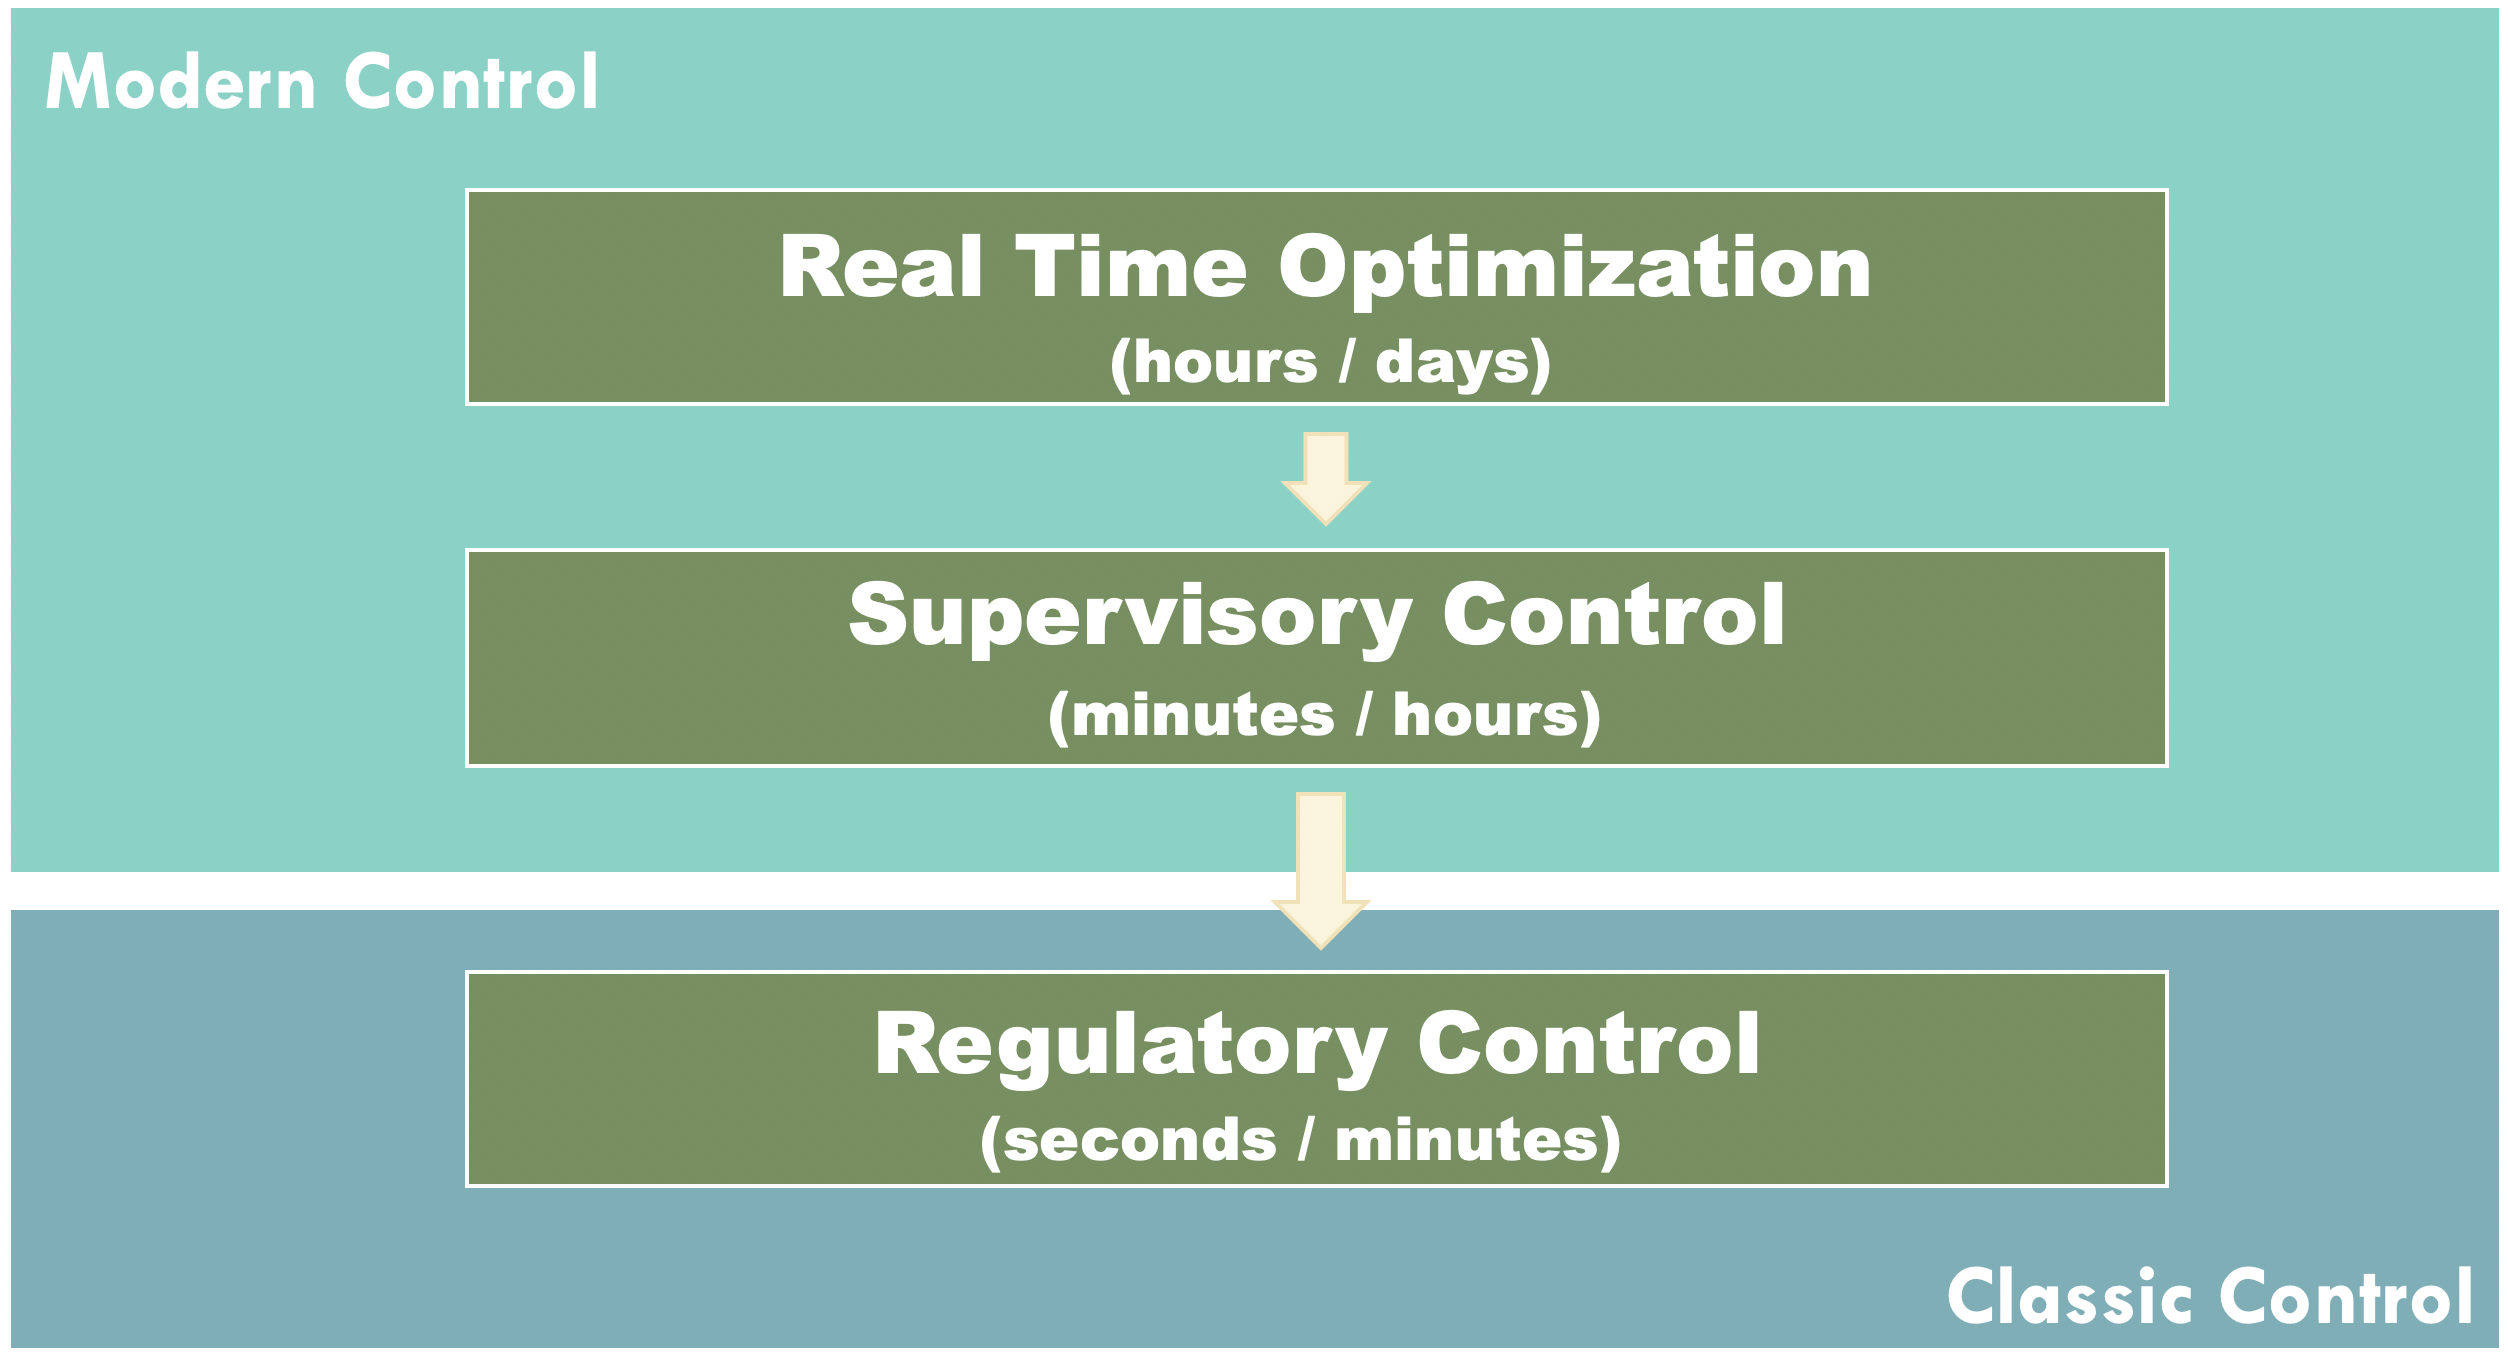
\includegraphics[scale=0.15]{images/08APC.png}
    \caption{Hierarchy of a typical control system.}
    \label{fig:08APC}
\end{figure}

\subsection{Problem Description}
Figure \ref{fig:08schedule} shows the communication framework of the pipeline operation. The goal of this pipeline is to meet the demands of the Commerce City refinery. To do so, a schedule with desired flow rates are sent to the operators from the scheduling team, and the operators are tasked to operate the pipeline at the given flow rate. Due to the complexity of this pipeline, different operators operate the pipeline differently even when the desired flow rate might be identical.  This difference introduces turbulence and unnecessary wear-and-tear onto the pipeline, increasing maintenance costs. 

\begin{figure}[h]
    \centering
    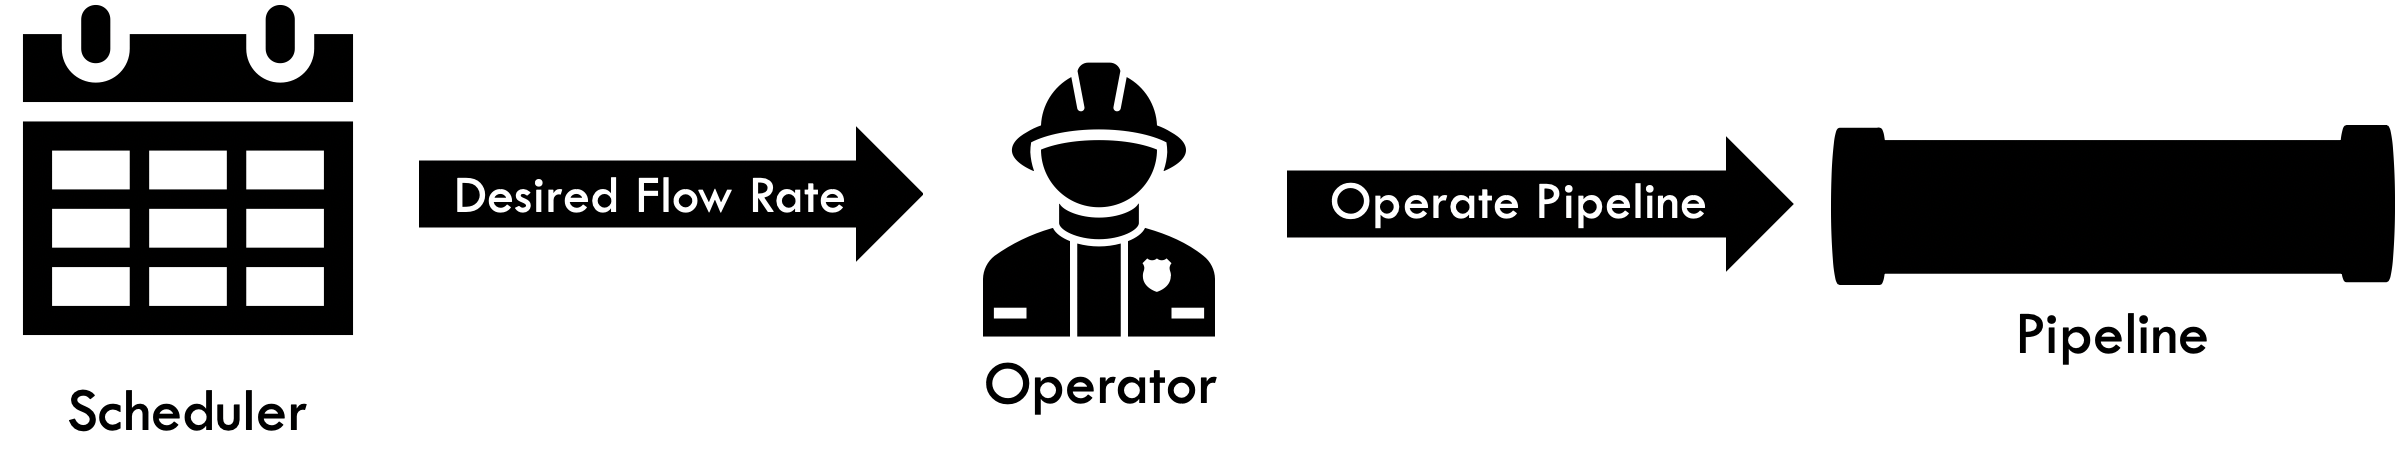
\includegraphics[scale=0.35]{images/08Schedule.png}
    \caption{Communication framework for operating line RM06A.}
    \label{fig:08schedule}
\end{figure}

To overcome this problem, machine learning was used to firstly identify a model of the pipeline.  Then, a steady state optimization tool was built using mixed integer linear programming to give operators the \textbf{optimal} set-points for each equipment.  This system solves two problems: i) Introduces uniformity in operator behaviour for desired set-points. ii) Semi-automation of the pipeline, freeing up operators' time for other tasks.

The new communication framework for line RM06A is shown in Figure \ref{fig:08scheduleV2}.

\begin{figure}[h]
    \centering
    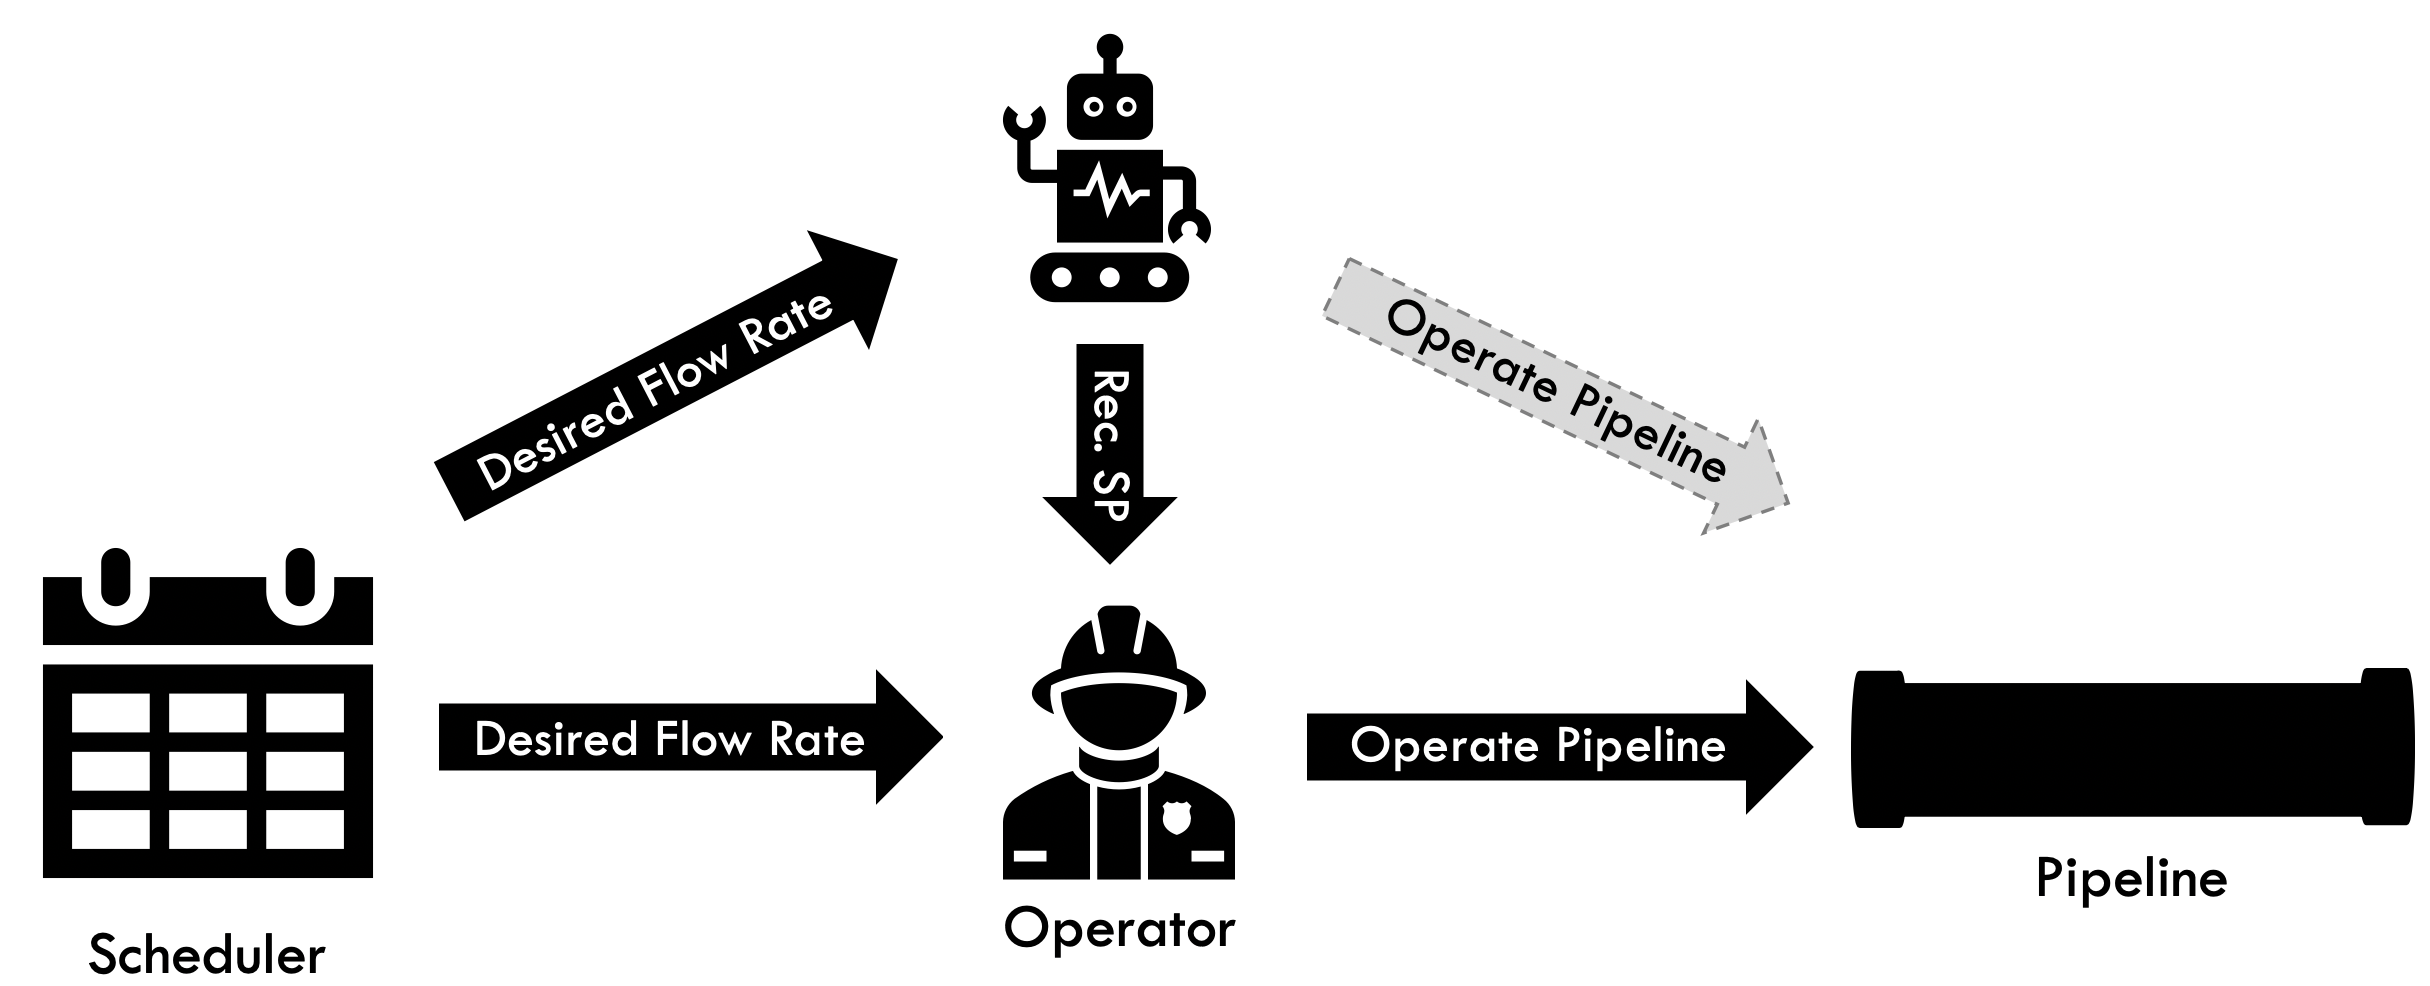
\includegraphics[scale=0.35]{images/08ScheduleV2.png}
    \caption{Proposed communication framework for operating line RM06A.}
    \label{fig:08scheduleV2}
\end{figure}

The rest of the section is as follows.  First, the data pre-processing step will be shown.  Then, the model identification phase will be introduced.  Following that, the optimization algorithm and all it's constraints for real-time optimization are presented.  Finally, the section is concluded with some conceptual software design regarding its implementation into a supervisory control and data acquisition (SCADA) system and the overall project impact will also be shown.

\subsection{Data Pre-processing}
Two data sets were provided by Suncor.  The details are shown in Table \ref{tab:08data}. Model identification and optimization evaluations were conducted for both datasets; however, the steps are very similar.  Because the 2019 algorithm will go into live production, whereas the 2018 data was used primarily as a proof of concept, only the 2019 algorithm steps will be shown in detail.

\begin{table}[h]
    \centering
    {\setstretch{1.5}
    \begin{tabular}{ c | c }
        Date of Collection     &      Data Dimension      \\
        \hline
        June 2017 - June 2018  &    $525,601 \times 899$   \\
        Dec. 2018 - March 2019 &    $159,851 \times 738$   \\
    \end{tabular}}
    \caption{Suncor data details.}
    \label{tab:08data}
\end{table}

Data pre-processing can be broken down into three phases: Filtering by subject matter experts, automated data pre-processing, and manual data pre-processing.  An iterative procedure followed phase three where the subject matter experts worked alongside the machine learning scientists to give suggestions on which variables should be included/excluded in the final model.

\subsubsection{Filtering by Subject Matter Experts}
The first phase of data pre-processing was conducted by the subject matter experts at Suncor.  The original data set contained all data corresponding to the pipeline.  Variables such as alarm limits, fire detector status, monitor on/off status, etc., have low predictive power and were removed.  After this phase, the number of variables reduced from 738 to 124.  

The distribution of the remaining variables along the pipeline can be seen in Table \ref{tab:08Ph1Data}.

\begin{table}[h]
    \centering
    {\setstretch{1.5}
    \begin{tabular}{ c | c | c | c | c | c | c}
             &  Cheyenne & CIG & Ault & Fort Lupton & Comm. City & Other      \\
        \hline
        \# of Variables  &  24  &  21  &  21  &  33  &  22  &  3  \\
    \end{tabular}}
    \caption{Distribution of variables along line RM06A after phase 1 data pre-processing.}
    \label{tab:08Ph1Data}
\end{table}

\subsubsection{Automated Data Pre-processing}
Next, the data set is further filtered using the following methods:

\begin{itemize}
    \item \textbf{Missing data removal}: Remove \textit{rows} of data containing missing data.
    \item \textbf{Data imbalance analysis}: Remove boolean variables that contain 97\% or more of a single class.  Heavily imbalanced variables cause model bias towards the majority class \cite{data_preprocessing}.
    \item \textbf{Collinear analysis}: Identifies variables that are correlated over 90\%. Correlation, $r_{xy}$ is given in Equation \ref{eq:08correlation}. One variable is kept while the rest are removed to prevent one variable from being weighed many times in the final model \cite{data_preprocessing}.
    \begin{equation}
        r_{xy} = \frac{\sum(x_i - \bar{x})(y_i - \bar{y})}{\sqrt{\sum(x_i - \bar{x})^2\sum(y_i-\bar{y})^2}}
        \label{eq:08correlation}
    \end{equation}
    
\end{itemize}

This phase is known as \textit{automated} because no human interaction and/or expertise is required. After performing the above methods, the data set reduced from 124 to 65.  

The distribution of the new data set is shown in Table \ref{tab:08Ph2Data}.

\begin{table}[h]
    \centering
    {\setstretch{1.5}
    \begin{tabular}{ c | c | c | c | c | c | c}
             &  Cheyenne & CIG & Ault & Fort Lupton & Comm. City & Other      \\
        \hline
        \# of Variables  &  10  &  11  &  11  &  18  &  12  &  3  \\
    \end{tabular}}
    \caption{Distribution of variables along line RM06A after phase 2 data pre-processing.}
    \label{tab:08Ph2Data}
\end{table}

\subsubsection{Manual Data Pre-processing}
Finally, the data set is then manually pre-processed to modify data from badly behaving sensors and irregular operating conditions.  In this phase, only the number of training examples where be reduced.

For this pipeline, both sweet and sour crude are transported in a cyclical fashion due to the hydraulic dynamics of the pipeline. Otherwise, the sour crude is too heavy to be transported for sustainable periods. However, downstream demand for each product can disrupt this operating cycle.  From Figure \ref{fig:08API}, it can be seen that there were extended periods of time where only sweet or sour crude were being transported, and was caused by the lack of demand downstream.  Such scenarios deviate from normal operations and were removed from the data.

\begin{figure}[h]
     \centering
     \begin{subfigure}[b]{1.0\textwidth}
         \centering
         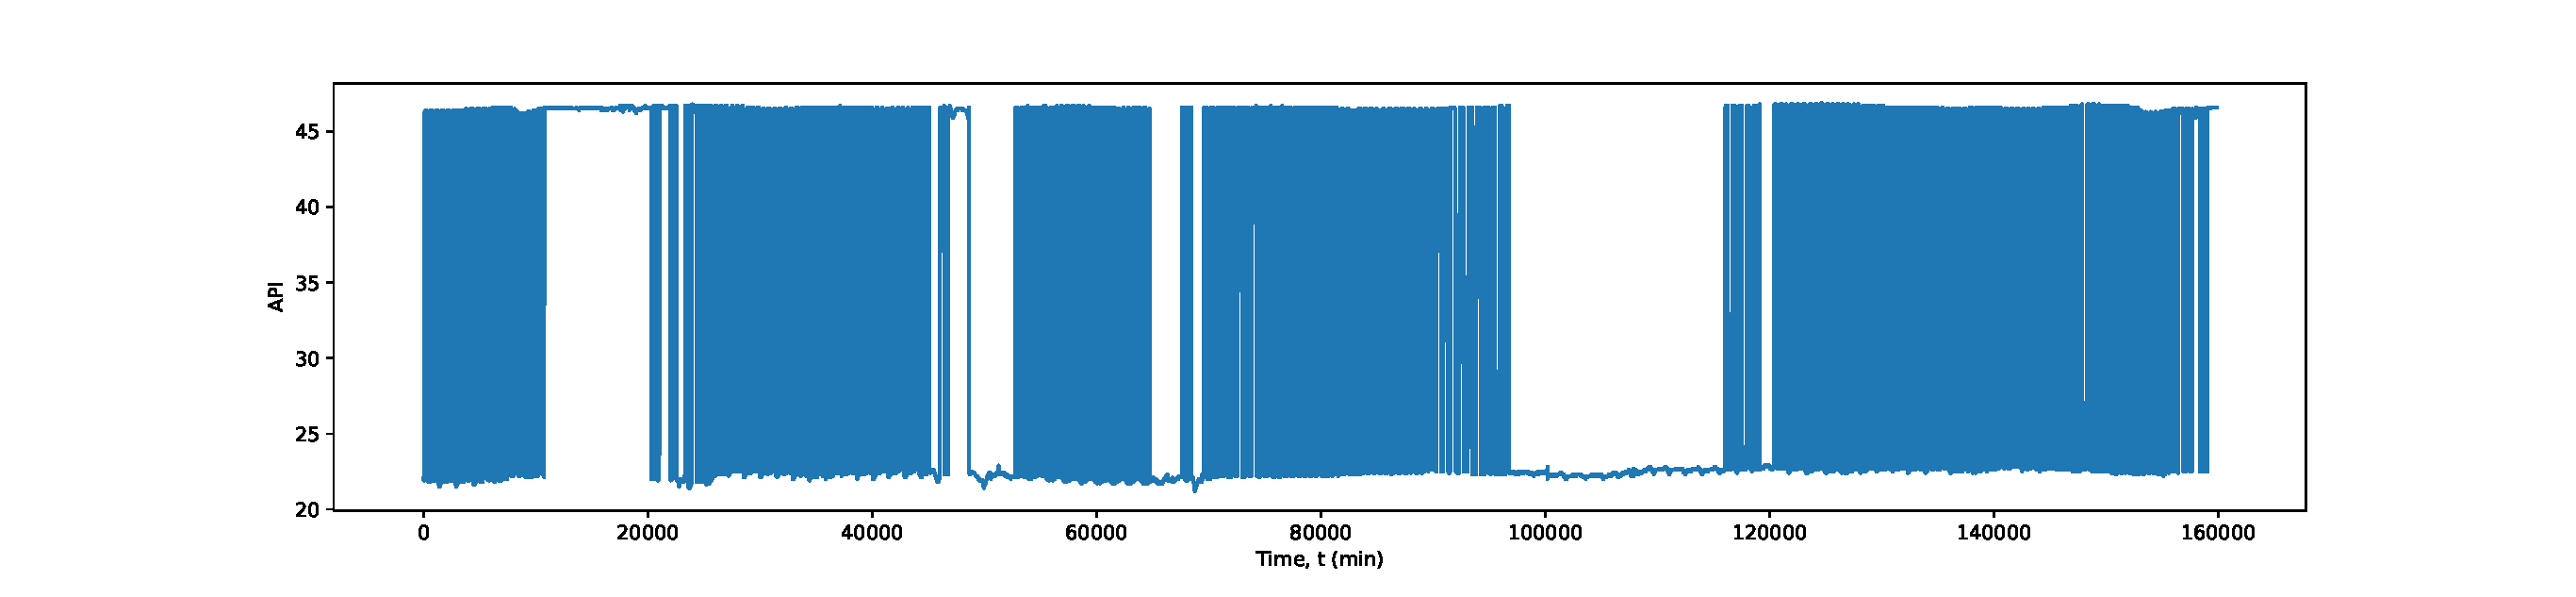
\includegraphics[width=\textwidth]{images/08NonFilteredDensity.eps}
         \caption{API data before abnormal condition removal.}
         \label{fig:08APIBefore}
     \end{subfigure}
     \hfill
     \begin{subfigure}[b]{1.0\textwidth}
         \centering
         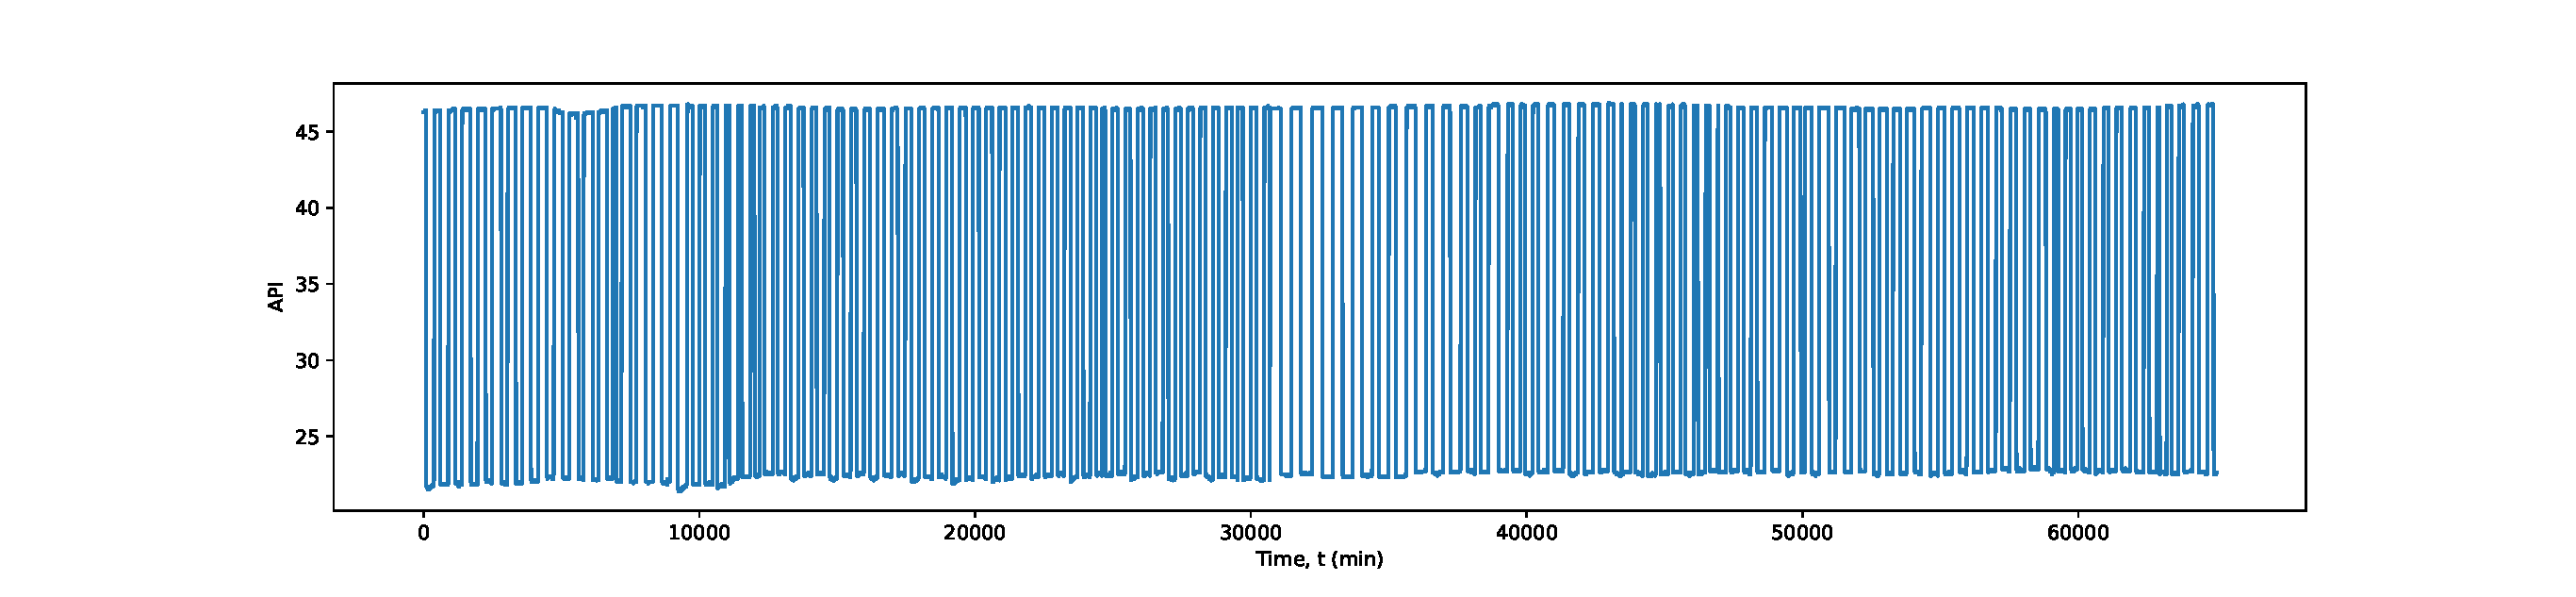
\includegraphics[width=\textwidth]{images/08FilteredDensity.eps}
         \caption{API data after abnormal condition removal.}
         \label{fig:08APIAfter}
     \end{subfigure}
        \caption{API data before and after removing abnormal operating conditions.}
        \label{fig:08API}
\end{figure}

Moreover, when a DRA set point is changed, there is a time delay for the flow rate to react because the new DRA concentration must be transported throughout the line before its effect can be fully realized.  DRA is catastrophically destroyed when passing through a pump; thus, DRA is only required to coat the pipeline between pump stations for its full effect to be exploited.  For CIG, it must coat the pipeline between CIG to Ault.  For Ault, the pipeline spanning between Ault and Fort Lupton must be coated.  Given the flow rate of the pipeline, it will take approximately ten hours to sufficiently coat the majority of the pipeline. Hence, data corresponding to transitional periods when DRA set points change are removed. At times, it may take longer; however, removing additional data will reduce the available data for identification of the machine learning models.  

Pre- and post-processed DRA parts per million (ppm) measurements are shown in Figure \ref{fig:08DRA}. DRA ppm is measured continuously for the control of the DRA injection pumps. However, the measurement is very difficult, unreliable and corrupted with noise. Because DRA set points are rarely changes, an exponentially weighted moving average (EWMA) was applied to the DRA ppm readings for increased measurement reliability.  The EWMA formula and bias correction are given in Equations \ref{eq:08EWMA} and \ref{eq:08Bias_Correction}, respectively: 
\begin{equation}
    v_t = \beta v_{t - 1} + (1 - \beta) \theta_t, \; v_0 = 0
    \label{eq:08EWMA}
\end{equation}
\begin{equation}
    v_t \leftarrow \frac{v_t}{1 - \beta^t}, \forall v \in V
    \label{eq:08Bias_Correction}
\end{equation}
where $v_{t}$ is the exponentially weighted value at time $t$.  $\beta$ is the exponentially weighing factor.  Larger $\beta$ results in smoother results.  $\theta_t$ is the original value at time $t$. $V$ is a vector representing the exponentially weighted values before bias correction.

\begin{figure}
     \centering
     \begin{subfigure}[b]{0.9\textwidth}
         \centering
         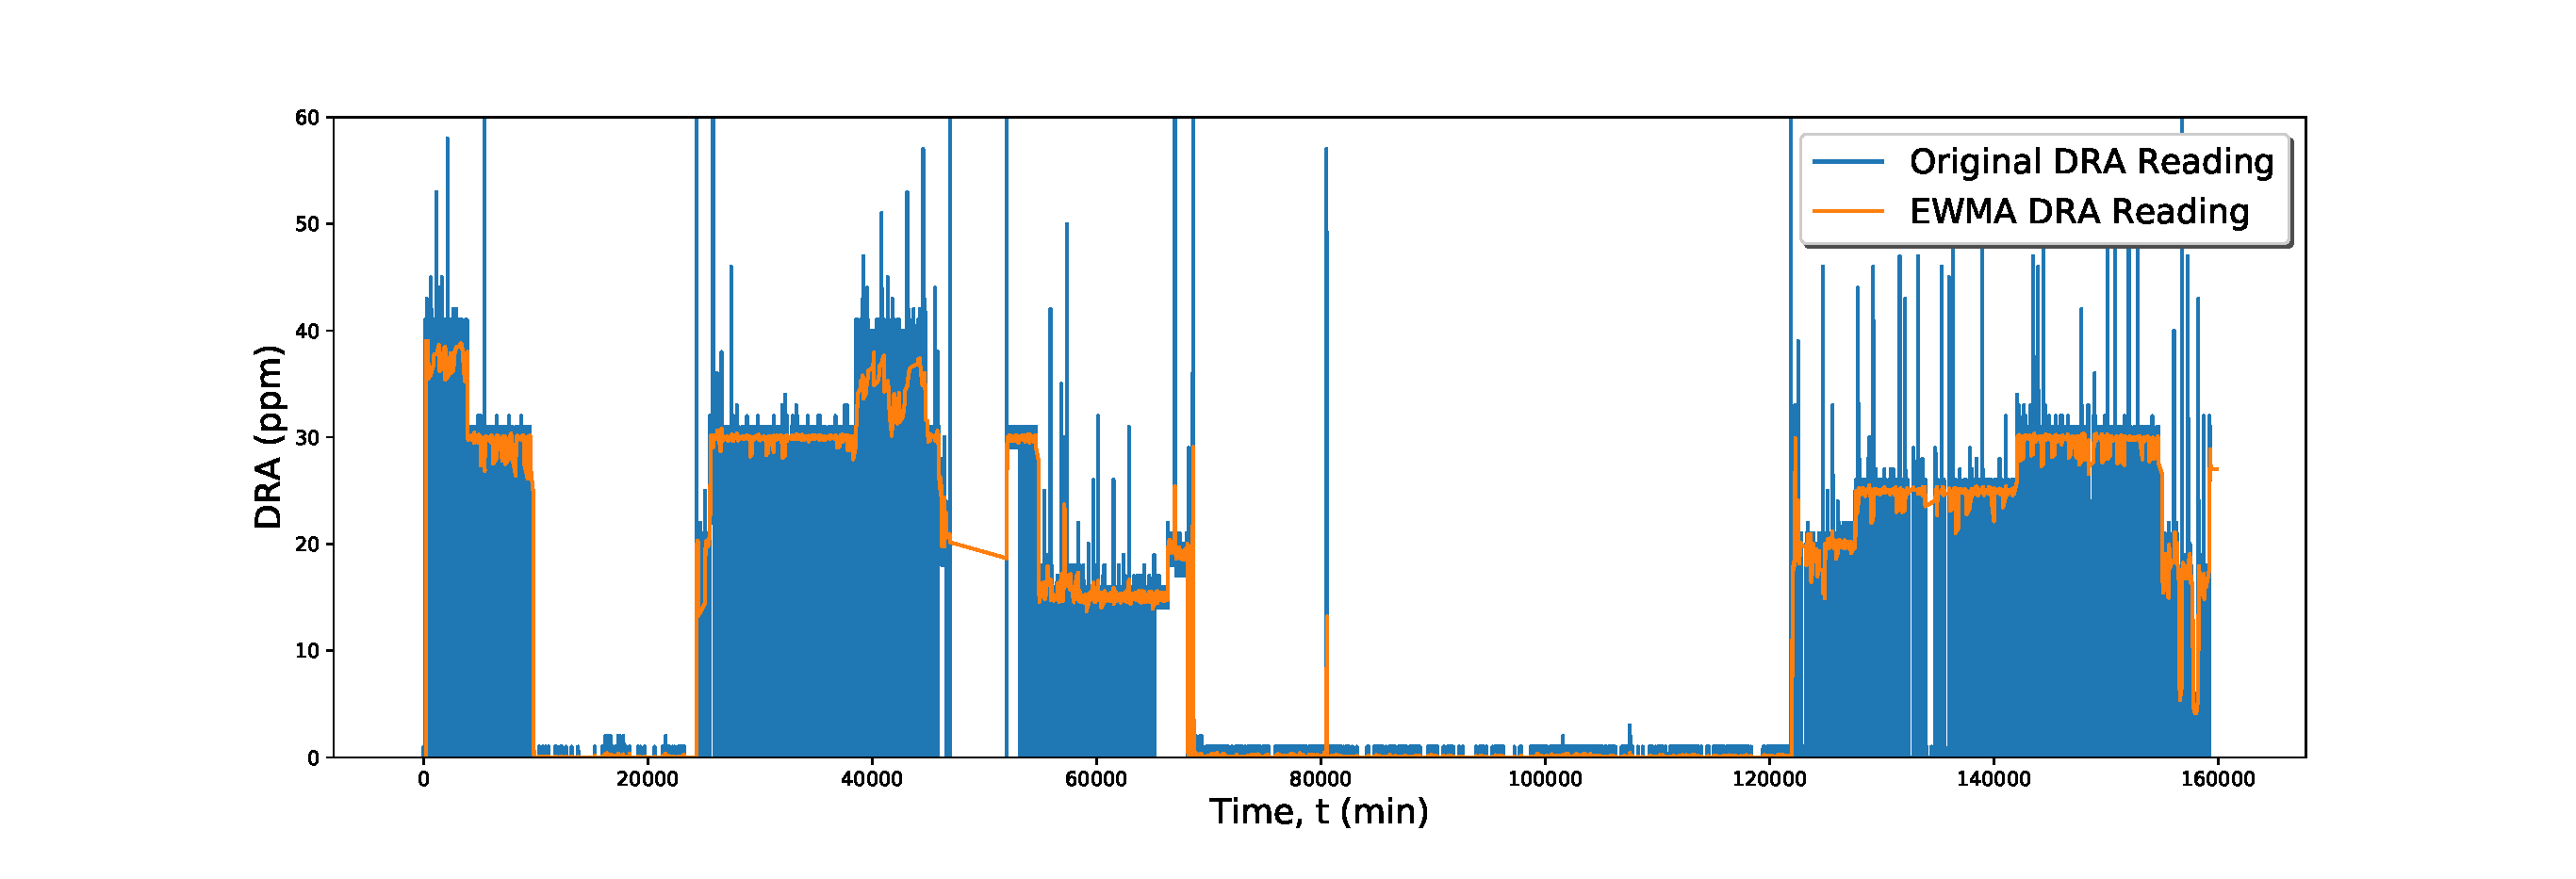
\includegraphics[width=\textwidth]{images/08CIGSour.eps}
         \caption{CIG sour DRA sensor reading.}
         \label{fig:08CIGSour}
     \end{subfigure}
     \begin{subfigure}[b]{0.9\textwidth}
         \centering
         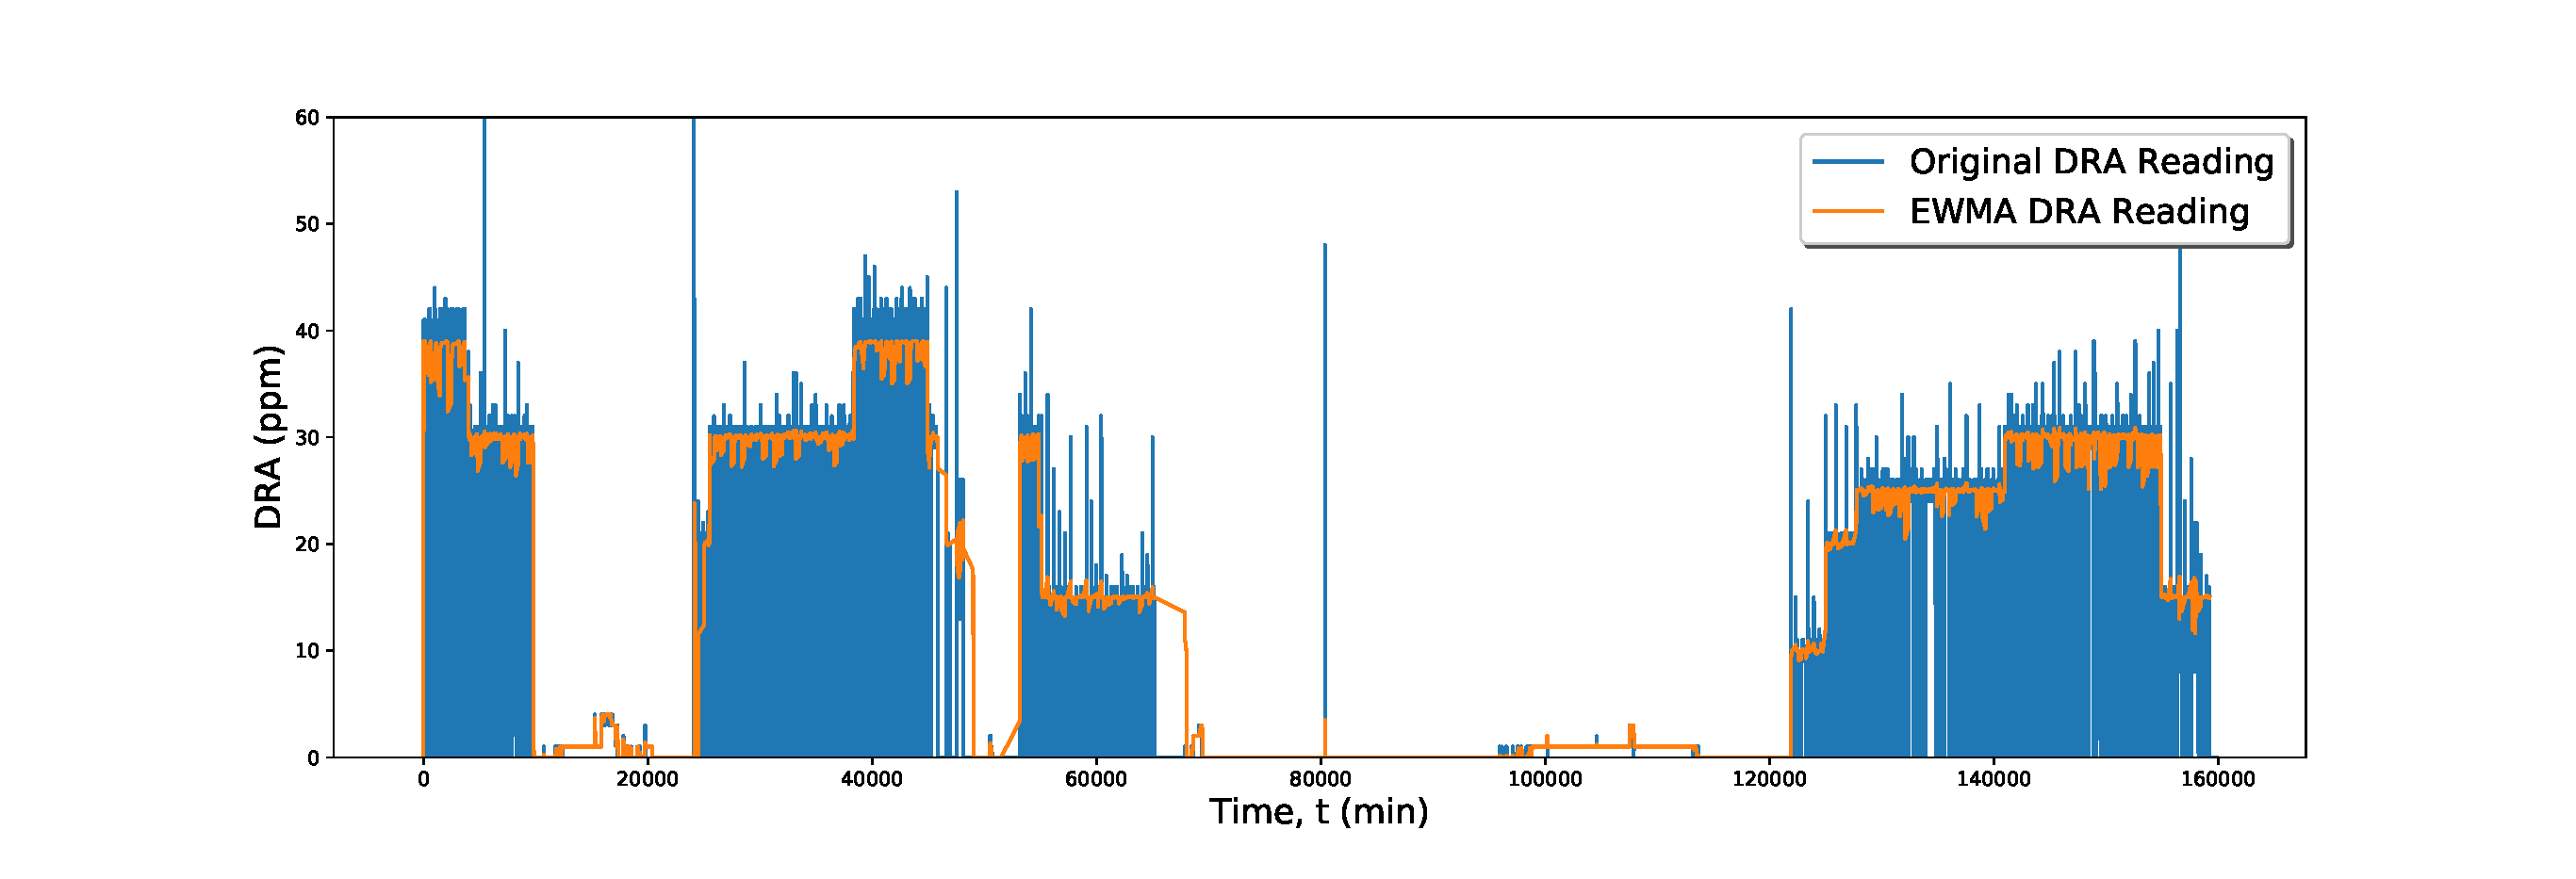
\includegraphics[width=\textwidth]{images/08CIGSweet.eps}
         \caption{CIG sweet DRA sensor reading.}
         \label{fig:08CIGSweet}
     \end{subfigure}
     \begin{subfigure}[b]{0.9\textwidth}
         \centering
         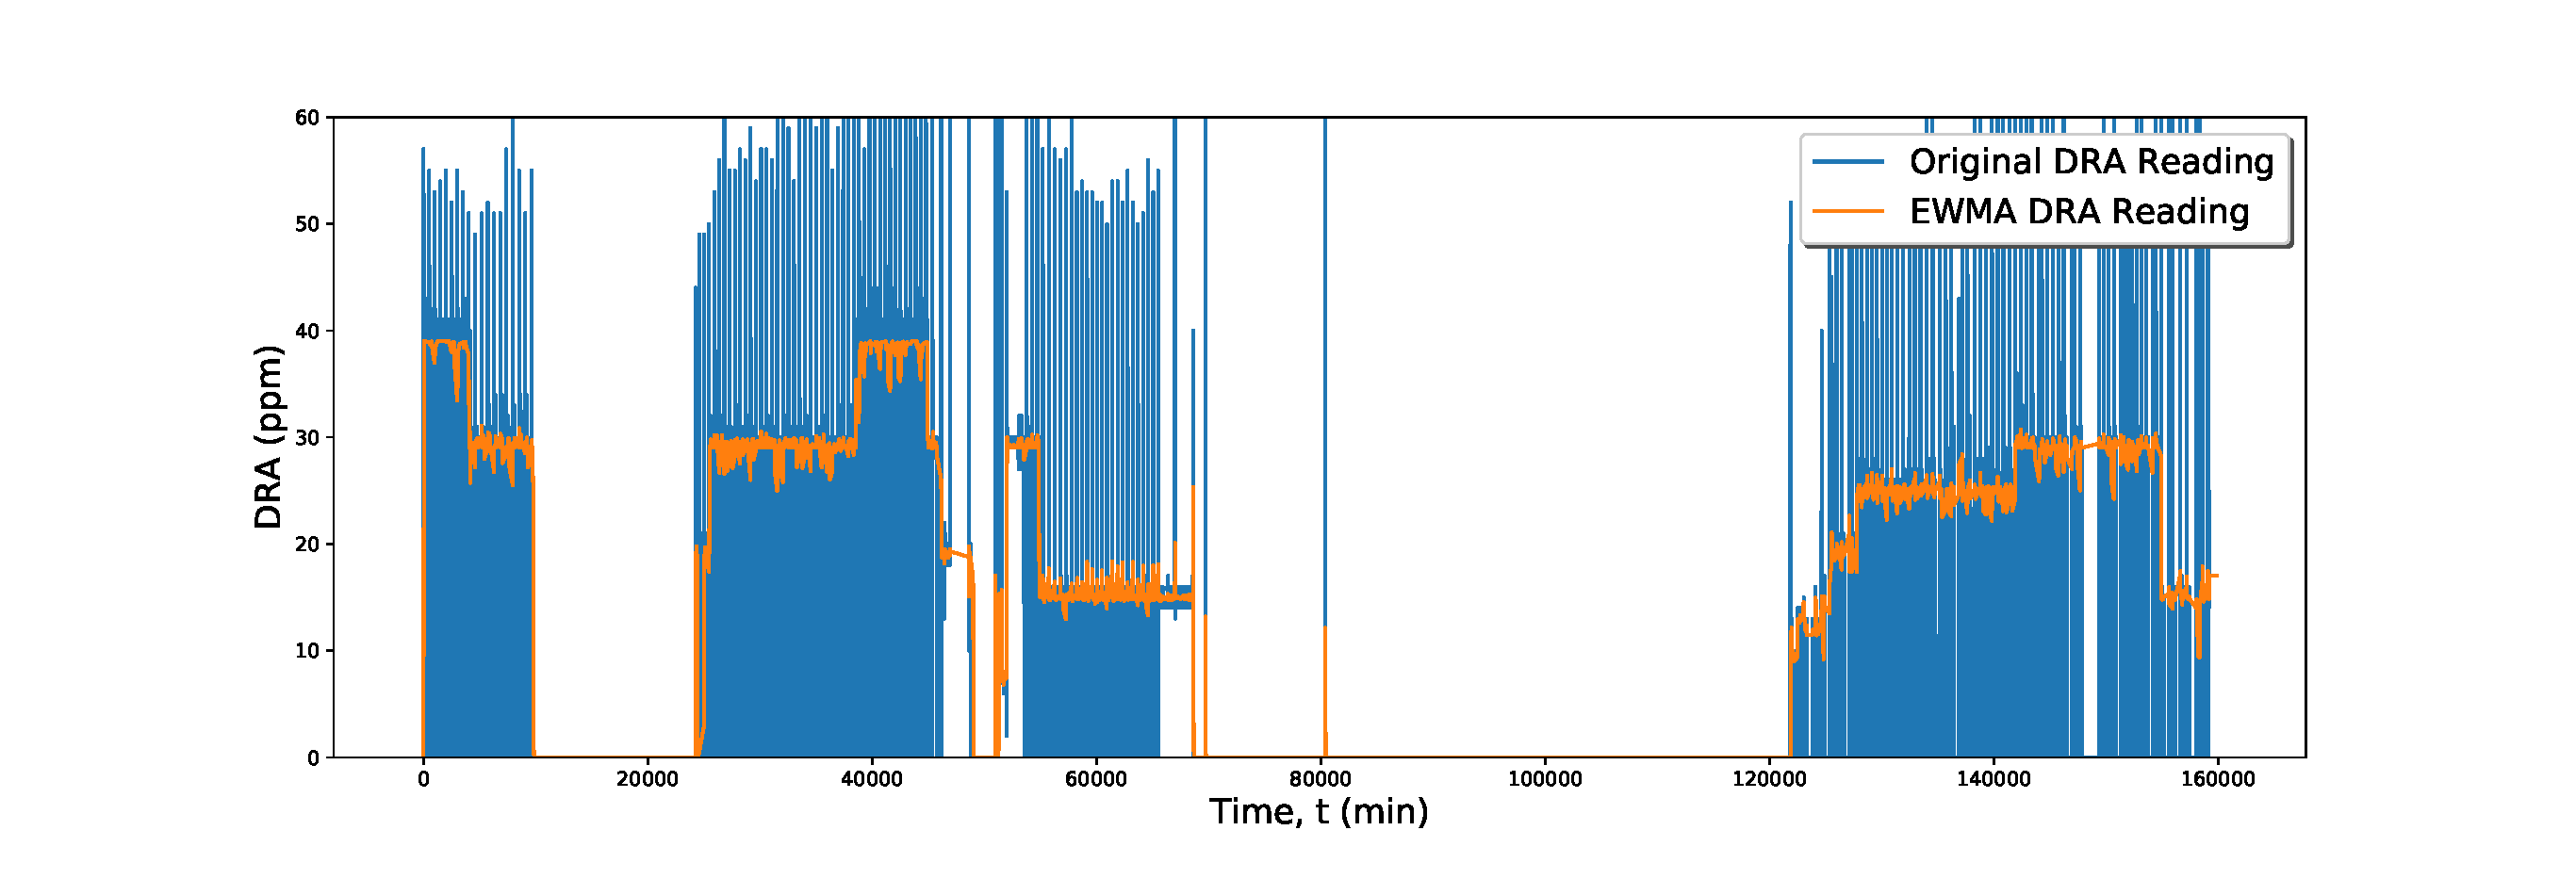
\includegraphics[width=\textwidth]{images/08AultSour.eps}
         \caption{Ault sour DRA sensor reading.}
         \label{fig:08AultSour}
     \end{subfigure}
     \begin{subfigure}[b]{0.9\textwidth}
         \centering
         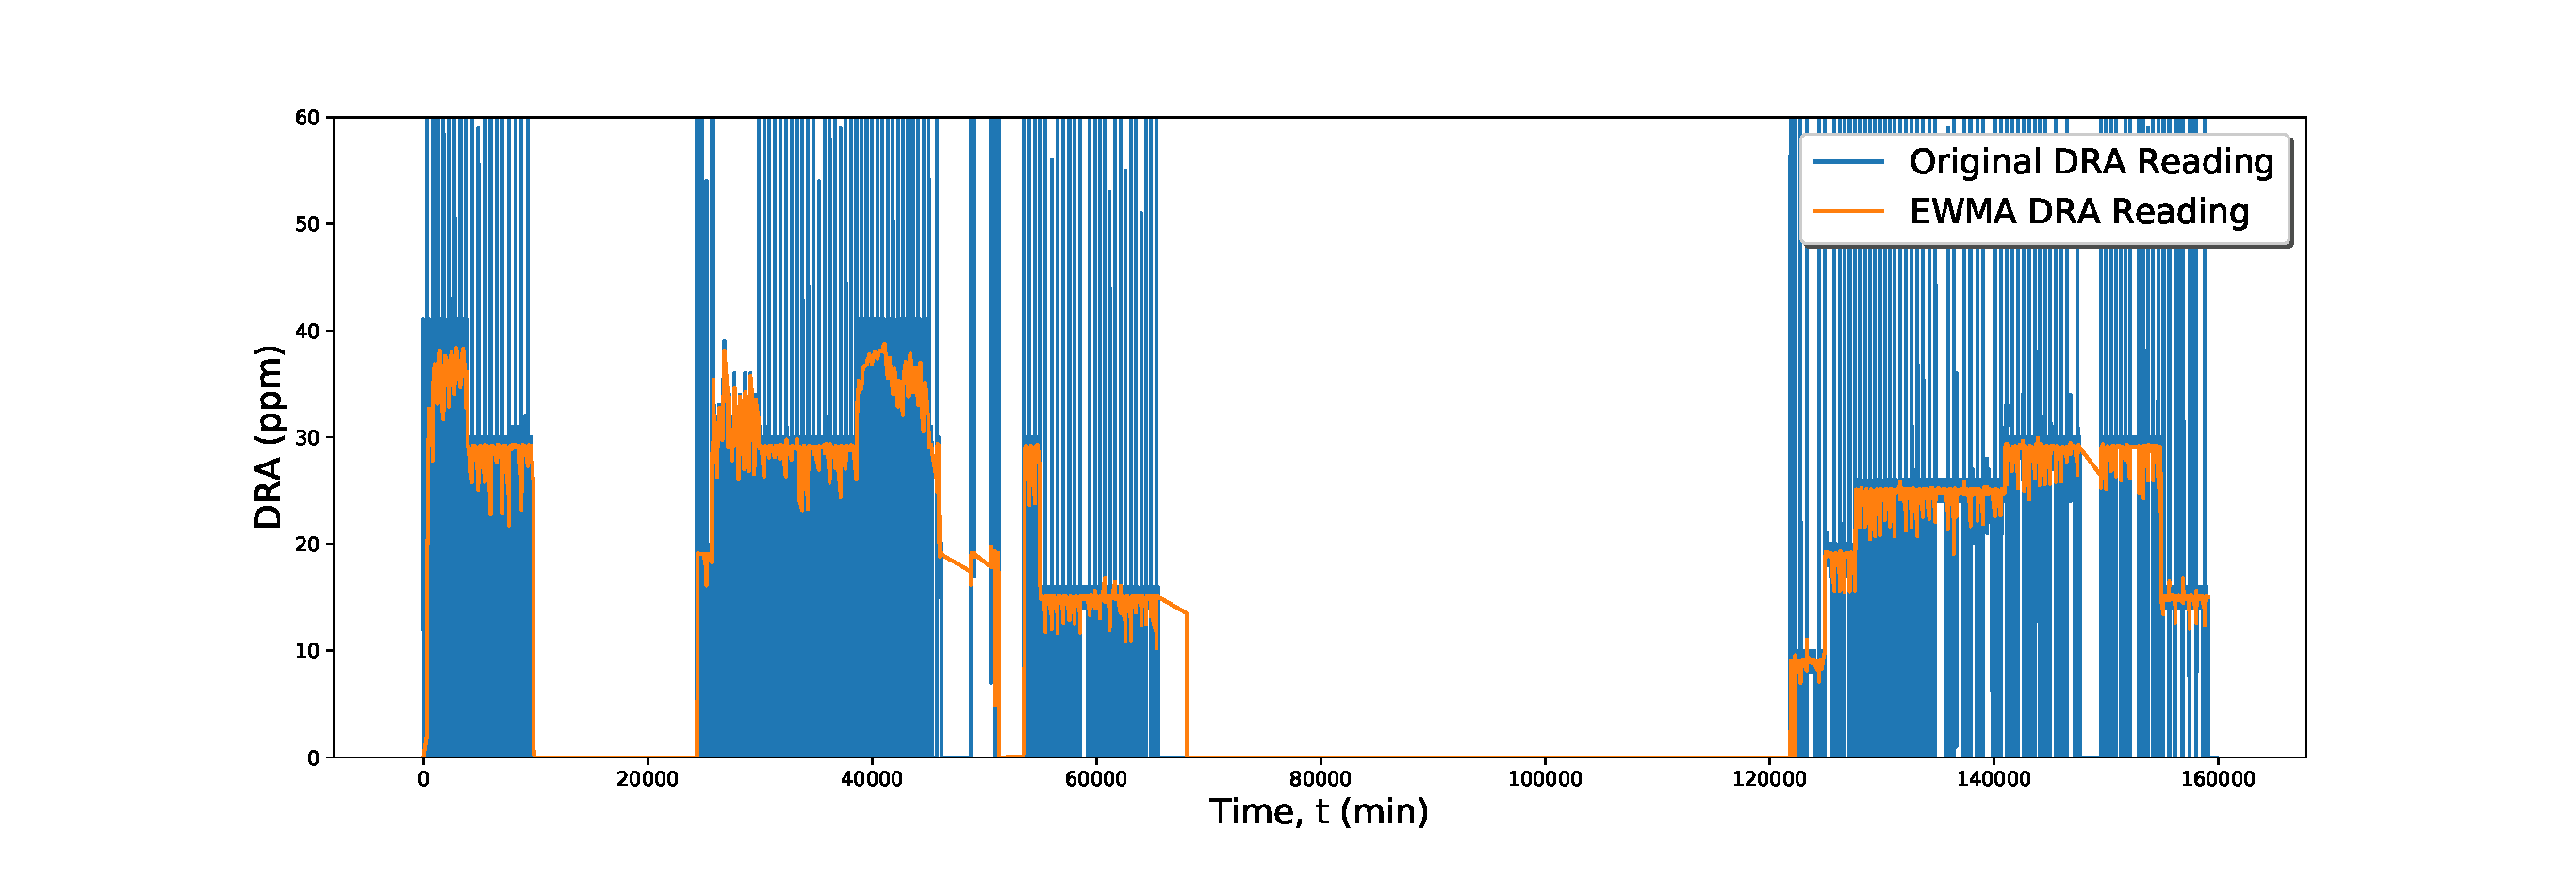
\includegraphics[width=\textwidth]{images/08AultSweet.eps}
         \caption{CIG sweet DRA sensor reading.}
         \label{fig:08AultSweet}
     \end{subfigure}
        \caption{Pre- and post-processed DRA sensor readings.}
        \label{fig:08DRA}
\end{figure}

Finally, the objective of the machine learning model was to predict the flow rate at Commerce City.  However, there is a natural time delay between the time an equipment status changed and the corresponding impact on downstream flow rate.  Because the pipeline is fully loaded and the product is incompressible, pressure changes upstream will be propagated downstream at close to the speed of sound \cite{fluid_mechanics}.  Table \ref{tab:08TimeToCC} shows the time required for pressure to propagate down the pipeline starting from each pump station.  The pump data for each pump station was shifted accordingly to account for this time delay, so predicted flow rates correspond to correct equipment configurations.  
\begin{table}[h]
    \centering
    {\setstretch{1.5}
    \begin{tabular}{ p{6cm} | c | c | c | c}
             &  Cheyenne & CIG & Ault & Fort Lupton \\
        \hline
        Time to Commerce City at speed of sound in liquids (1480 m/s) \cite{fluid_mechanics}
        &  1.7 min  &  1.5 min  &  1.0 min  &  0.45 min  \\
    \end{tabular}}
    \caption{Time required for pressure changes at each pump station to be realized at Commerce City.}
    \label{tab:08TimeToCC}
\end{table}
A comprehensive list of the manual data pre-processing procedures is as follows:
\begin{enumerate}
    \item Shift data to accommodate the time delay at Commerce City.
    \item Smooth DRA data using exponentially weighted moving average given in Equation \ref{eq:08EWMA}.  
    \item Remove first 10 hours data corresponding to DRA set point changes.
    \item Remove data points where flow is under 800 bbl/hr.
    \item Remove data when only sweet or sour crude was sent through the pipeline.
\end{enumerate}

The final data set contained 65 variables and 97,470 data points.

\subsection{Model Identification}
\subsubsection{Feature Selection}
For each pump station, there was a variety of sensors measuring the same process variables at different locations.  For example, VFD pumps have four readings each: On/off status, RPM, HZ, and current. Many variables relating to one equipment is redundant; thus, only one variable was selected when redundancy existed. Additionally, some sensors were behaving abnormally.

In normal operations, the density fluctuates between 10 - 50 API, depending on the type of crude present in the pipeline.  After analysis, the Fort Lupton densitometer was behaving abnormally compared to other densitometer and is shown in Figure \ref{fig:08Density}.  After confirming with Suncor that the densitometer was behaving abnormally, the variable was removed.  
\begin{figure}[h]
     \centering
     \begin{subfigure}[b]{0.48\textwidth}
         \centering
         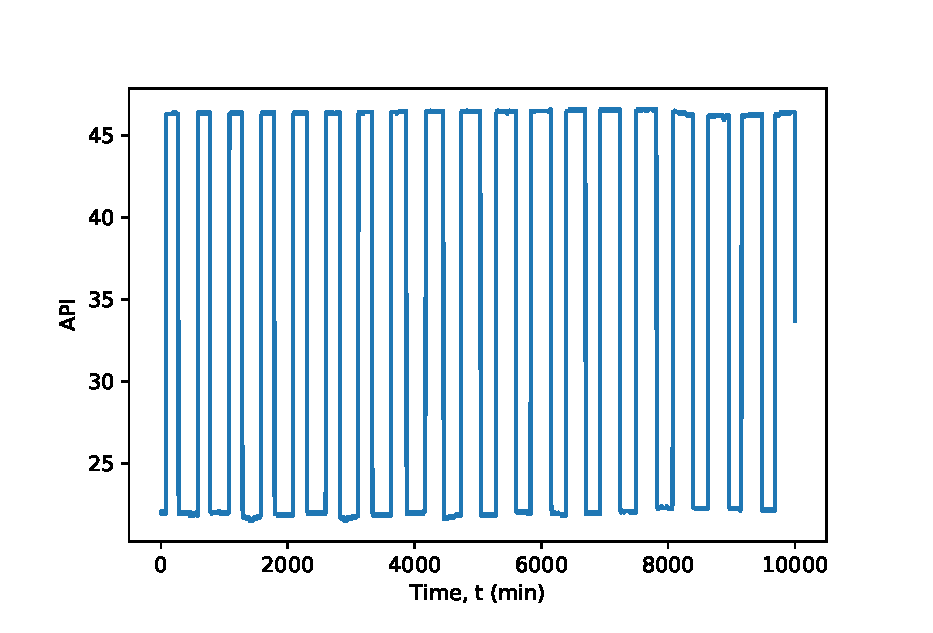
\includegraphics[width=\textwidth]{images/08CheyDensity.eps}
         \caption{Cheyenne API data for 10,000 mins.}
         \label{fig:08GoodDensity}
     \end{subfigure}
     \hfill
     \begin{subfigure}[b]{0.48\textwidth}
         \centering
         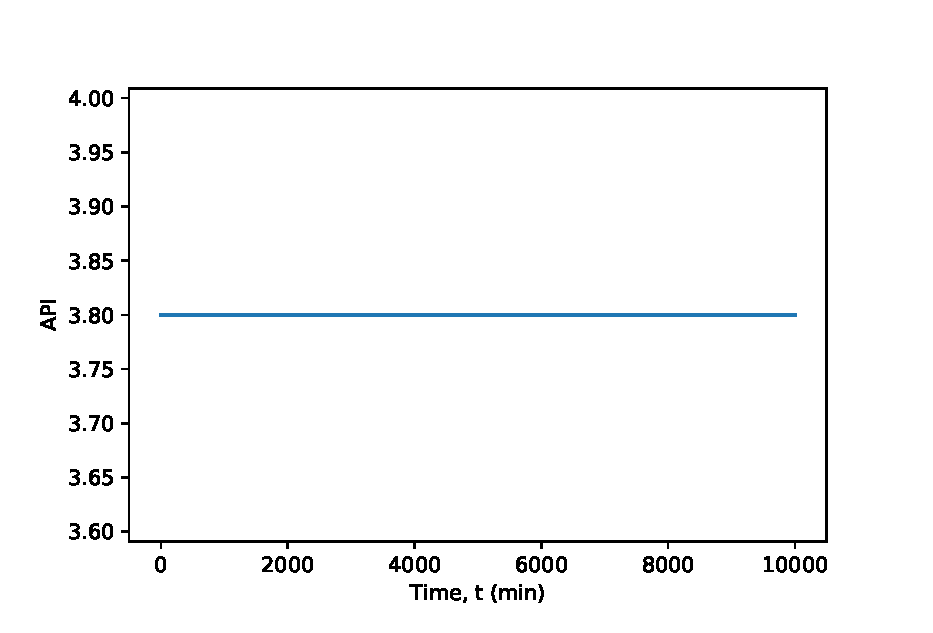
\includegraphics[width=\textwidth]{images/08FLDensity.eps}
         \caption{Fort Lupton API data for 10,000 mins.}
         \label{fig:08BadDensity}
     \end{subfigure}
        \caption{Comparison of normal and abnormal density readings.}
        \label{fig:08Density}
\end{figure}

Table \ref{tab:08featselect} shows the features selected for each pump station. The predicted variable was the flow rate (bbl/h) at Commerce City.
\begin{table}[h]
    \centering
    {\tiny
    {\setstretch{1.5}
    \begin{tabular}{ c | c | c | c | c}
        Cheyenne                       & CIG                      & Ault                        & Fort Lupton                    & Commerce City \\
        \hline
        $x_5$: Boos. Pump Status       &  $x_1$: Sweet DRA (ppm)  &  $x_3$: Sweet DRA (ppm)     &  $x_{8}$: Boos. Pump Status   &  $x_{18}$: Inlet Temp. (°C) \\
        
        $x_9$: VFD Current (Amp)       &  $x_2$: Sour DRA (ppm)   &  $x_4$: Sour DRA (ppm)      & $x_{10}$: VFD Current (Amp)      & \\
        
        $x_{14}$: Inlet Temp. (°C)     &  $x_{15}$: Inlet Temp. (°C) &  $x_6$: Small Pump Status &  $x_{17}$: Inlet Temp. (°C)  & \\
        
        $x_{11}$: API                   &  $x_{12}$: API          &  $x_7$: Large Pump Status   &             
        & \\
        
                                       &                          &  $x_{16}$: Inlet Temp. (°C)  &             
        & \\
        
                                       &                          &  $x_{13}$: API               &       
        & \\
        
    \end{tabular}}}
    \caption{Features selected for machine learning models.}
    \label{tab:08featselect}
\end{table}

\subsubsection{Feature Scaling}
Figure \ref{fig:08featscale} shows the contour of a normalized and non-normalized cost function. It can be seen that the optimization of a non-normalized cost function can be significantly hindered depending on where the optimization is initialized.

\begin{figure}[h]
    \centering
    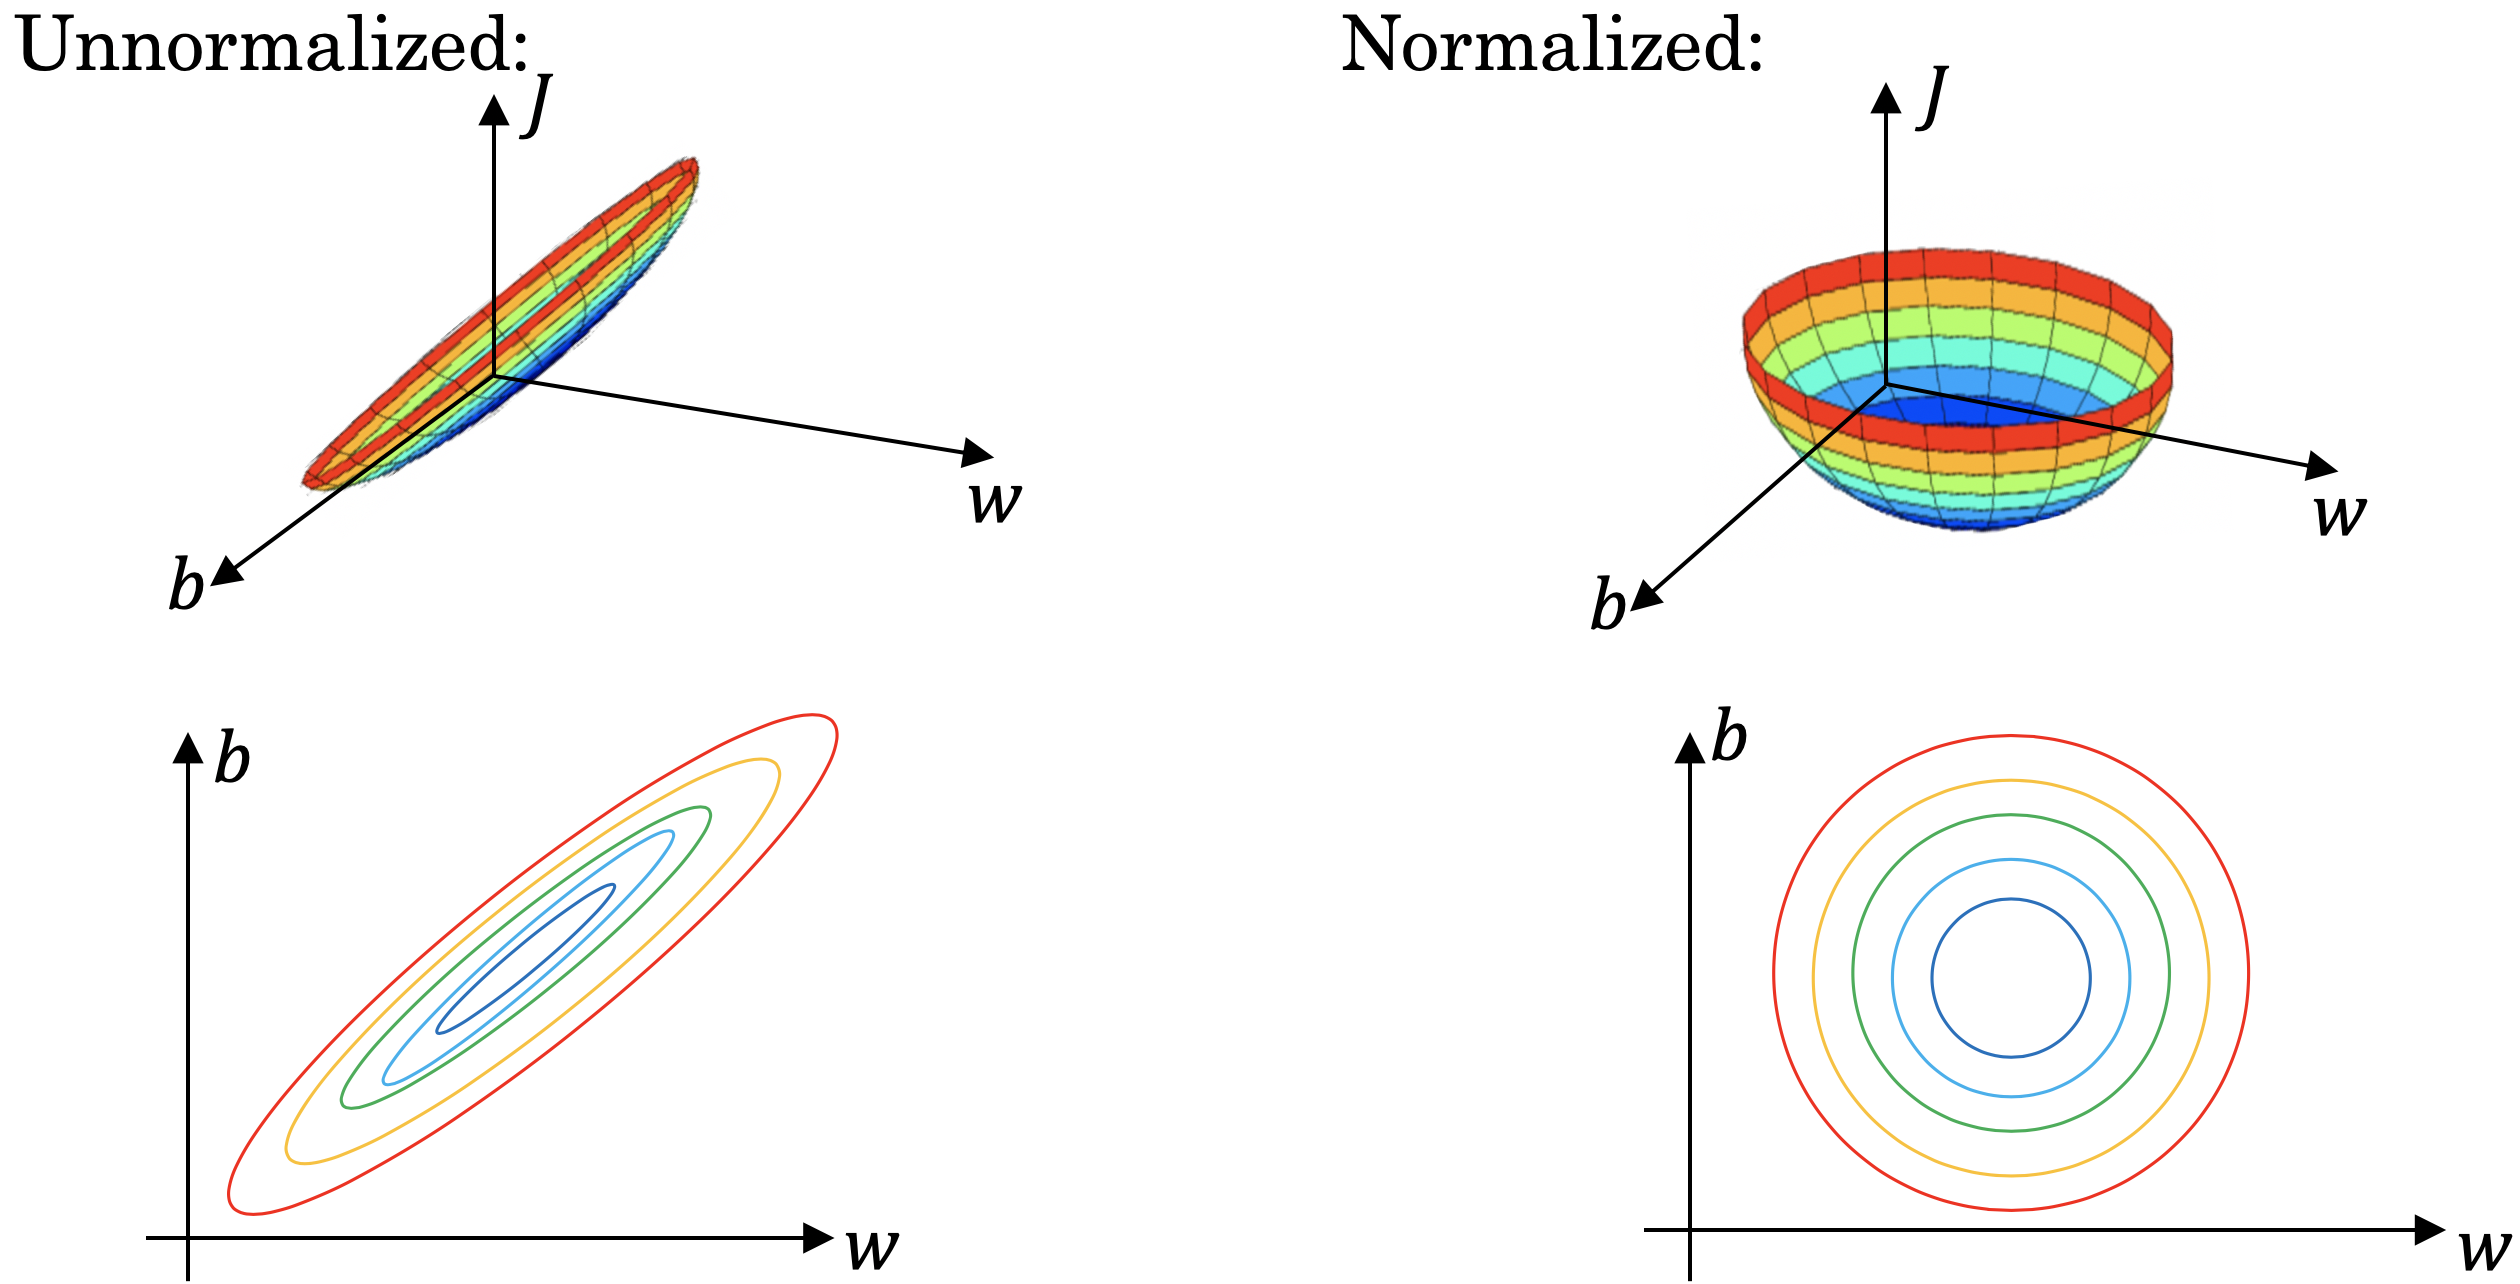
\includegraphics[width=1\textwidth]{images/08featscale.png}
    \caption{Coutour of normalized and non-normalized cost functions. Original images from \cite{deeplearning_course}.}
    \label{fig:08featscale}
\end{figure}

To avoid this problem, the min-max normalization is applied to each variable and is given by:
\begin{equation}
    x^{norm} = \frac{x - x^{min}}{x^{max} - x^{min}}
\end{equation}
where $x^{norm}$ is the normalized values.  Here, $x^{min}$ and $x^{max}$ are the minimum and maximum values of each variable, respectively.  By applying this normalization, all data are bounded between $x_i \in [0, 1]$, and the elongation issue of the cost function can be resolved.

\subsubsection{Exploratory Data Analysis}
- Bi-modal distribution
- Clustering analysis
  - Average characteristics
- Other characteristics for other variables.


\subsubsection{Data Partitioning}
The data set was split into three sections to validate and test the machine learning models: training, validation, and testing.  The partition and description of each section is described in Table \ref{tab:08datapart}. The training data set is used to identify the machine learning model(s).  Then, the model is validated on un-trained data via the validation data set (sometimes called development data).  The error of the model on the validation data set, $e_{validation}$, should be similar to the training data error, $e_{train}$, to ensure that the model did not overfit to the training data. Finally, the model will be tested on the testing data to explore the performance of the model in live production.
\begin{table}[h]
    \centering
    {\setstretch{1.5}
    \begin{tabular}{ c | c | p{9cm}}
                            & \% of Data        &  Description \\
        \hline
        Training            &  90\%             
        &  Used to identify the machine learning model        \\
        
        Validation          &  5\%              
        &  Validates the performance of the machine learning model         \\
        
        Testing             &  5\%             
        &  Used to test performance of machine learning model on unseen data       \\             
    \end{tabular}}
    \caption{Features selected for machine learning models.}
    \label{tab:08datapart}
\end{table}

\subsubsection{Cost Function}

For all predictive models, the mean squared error (MSE) cost function is used and is given by:
\begin{equation}
    J(W) = \frac{1}{n}\sum\limits^n_{i=1}(\hat{y}_i - y_i)^2
    \label{eq:08MSE}
\end{equation}
where $n$ is the number of samples in the current optimization step.  $\hat{y}_i$ and $y_i$ are the $i^{th}$ predicted and actual labels, respectively. Here, $J$ is the loss. The MSE cost function was selected due to its convex nature \cite{deeplearning_course}.

To ensure adequate performance on the validation and testing data, the model must avoid overfitting to the training data.  One common way to reduce model complexity is by removing or reducing individual variables' impact on the model.  This study used a ridge regularization to reduce model complexity:
\begin{equation}
    J(W) = \frac{1}{n}\sum\limits^n_{i=1}(\hat{y}_i - y_i)^2 + \lambda \sum\limits^n_{j=1} W_j^2
    \label{eq:08MSE_wR}
\end{equation}
where $\lambda$ is the regularization penalty.  Here, as $\lambda \rightarrow \infty$, $W \rightarrow 0$.  That is, the larger $\lambda$ is, the stronger the weights are penalized. 

\subsubsection{Model Optimization}

The adaptive momentum (ADAM) gradient descent optimizer was used to update the weights and bias of the models.  The general gradient descent formulation is given by Equation \ref{eq:08GradientDescent} \cite{ADAM}.  
\begin{equation}
    \theta_j^{m+1} \leftarrow \theta_j^{m} - \alpha \frac{\partial J}{\partial \theta_j}
    \label{eq:08GradientDescent}
\end{equation}
where $\theta_j$ is the $j^{th}$ weight of the model.  $m$ represents the $m^{th}$ update of gradient descent and $\alpha$ is the learning rate.  ADAM improves upon Equation \ref{eq:08GradientDescent} by computing an adaptive learning rate for each parameter. To do so, the exponentially decaying average of the past gradients and squared gradients of the weights and biases are computed and stored using Equations \ref{eq:08momentW} to \ref{eq:08squared_momentb}.
\begin{equation}
    V_{dW} = \beta_1 V_{dW} + (1 - \beta_1)dW
    \label{eq:08momentW}
\end{equation}
\begin{equation}
    V_{db} = \beta_1 V_{db} + (1 - \beta_1)db
    \label{eq:08momentb}
\end{equation}
\begin{equation}
    S_{dW} = \beta_2 S_{dW} + (1 - \beta_2)dW^2
    \label{eq:08squared_momentW}
\end{equation}
\begin{equation}
    S_{db} = \beta_2 S_{db} + (1 - \beta_2)db^2
    \label{eq:08squared_momentb}
\end{equation}
where $V$ and $S$ are the estimates of the gradient and squared gradients, respectively.  $V$ and $S$ are typically initiated as zero vectors and are heavily biased towards zero at initial steps.  Hence, the biases for the initial terms are corrected using:
\begin{equation}
    V_{dW}^{corrected} = \frac{V_{dW}}{1 - \beta_1^t}
\end{equation}
\begin{equation}
    V_{db}^{corrected} = \frac{V_{db}}{1 - \beta_1^t}
\end{equation}
\begin{equation}
    S_{dW}^{corrected} = \frac{S_{dW}}{1 - \beta_2^t}
\end{equation}
\begin{equation}
    S_{db}^{corrected} = \frac{S_{db}}{1 - \beta_2^t}
\end{equation}
Combining the above equations, the weights and biases are updated using ADAM by:
\begin{equation}
    W_j \leftarrow W_j - \alpha \frac{V_{dW}^{corrected}}{S_{dW}^{corrected} + \epsilon}
\end{equation}
\begin{equation}
    b \leftarrow b - \alpha \frac{V_{db}^{corrected}}{S_{db}^{corrected} + \epsilon}
\end{equation}
where $\epsilon$ is a small scalar to avoid division by zero. The authors proposed values of 0.9, 0.999 and $10^{-8}$ for $\beta_1$, $\beta_2$, and $\epsilon$, respectively.

Due to the size of the data, batch gradient descent where all data are used to compute the gradient at each step is computationally infeasible.  Thus, mini-batch gradient descent was used where smaller batches of data were sampled from the original data set to perform parameter updates at each step.
\subsubsection{Performance Assessment}
The model performance were assessed using the following three ways:
\begin{enumerate}
    \item Root mean squared error (RMSE):
    \begin{equation}
        J = \sqrt{\frac{1}{n}\sum\limits^n_{i=1}(\hat{y}_i - y_i)^2}
        \label{eq:08RMSE}
    \end{equation}
    
    \item Mean absolute error (MAE):
    \begin{equation}
        J = \frac{1}{n}\sum\limits^n_{i=1}|\hat{y}_i - y_i|
        \label{eq:08MSE_Error}
    \end{equation}
    \item Coefficient of determination ($R^2$):
    \begin{equation}
        R^2 = 1 - \frac{\sum\limits^n_{i = 1}(\hat{y_i} - y_i)^2}{\sum\limits^n_{i = 1}(y_i - \bar{y_i})^2}
    \end{equation}
\end{enumerate}
Table \ref{tab:08performanceassessment} shows the advantages and disadvantages of each assessment metric.
\begin{table}[h]
    \centering
    {\setstretch{1.5}
    \begin{tabular}{ c | p{7cm} | p{7cm}}
         Method             & Advantages        &  Disadvantages \\
        \hline
        RMSE                &  Useful for identifying large errors                            &  Smaller errors are more muted        \\
        
        MAE                 &  Easy to interpret as all errors have the same weight           &  Inferior to RMSE when large errors are undesirable \\
        
        $R^2$               &  Easy to understand, $0 \leq R^2 \leq 1$                                         &  Valid only for linear relationships       \\             
    \end{tabular}}
    \caption{Constrained least squares validation and test plots.}
    \label{tab:08performanceassessment}
\end{table}

%%%%%%%%%%%%%%%%%%%%%%%%%%%%%%%%%%%%%%%%%%%%%%%%%%%%%%%%%%%%%%%%%%%%%
%
% Least squares model
%
%%%%%%%%%%%%%%%%%%%%%%%%%%%%%%%%%%%%%%%%%%%%%%%%%%%%%%%%%%%%%%%%%%%%%

\subsubsection{Linear Modelling}
The least squares regression was the first regression method to be explored, and was selected as the benchmark due to its simplicity and linear nature. The model structure of least squares is given as:
\begin{equation}
    \hat{y} = W^Tx + b
    \label{eq:08LS}
\end{equation}
where $x$ is a vector of features and the superscript $T$ represents the transpose operation.

Hyper parameters of the linear regression are shown in Table \ref{tab:08LSHparameters}.
\begin{table}[h]
    \centering
    {\setstretch{1.5}
    \begin{tabular}{ c | c}
        Hyper Parameter                  &  Value       \\
        \hline
        Epochs                           &  800      \\
        Minibatch size                   &  8192     \\
        Learning rate, $\alpha$          &  0.001    \\
        Regularization, $\lambda$          &  0.001  \\
    \end{tabular}}
    \caption{Hyper parameters for least squares regression.}
    \label{tab:08LSHparameters}
\end{table}
The performance assessment of the least squares model is shown in Table \ref{tab:08LSperformance}.
\begin{table}[h]
    \centering
    {\setstretch{1.5}
    \begin{tabular}{ c | c | c | c}
                             &  Training data    &  Validation data   &    Test data      \\
        \hline
        MAE                  &  98               &    98              &  102     \\
        RMSE                 &  127              &   127              &  135    \\ 
        $R^2$                &  0.91             &   0.91             &  0.70   \\
    \end{tabular}}
    \caption{Performance assessment for the least squares model.}
    \label{tab:08LSperformance}
\end{table}
The model performance on the validation and test data sets are shown in Figures \ref{fig:08LSValidation} and \ref{fig:08LSTest}.
\begin{figure}[h]
     \centering
     \begin{subfigure}[b]{0.48\textwidth}
         \centering
         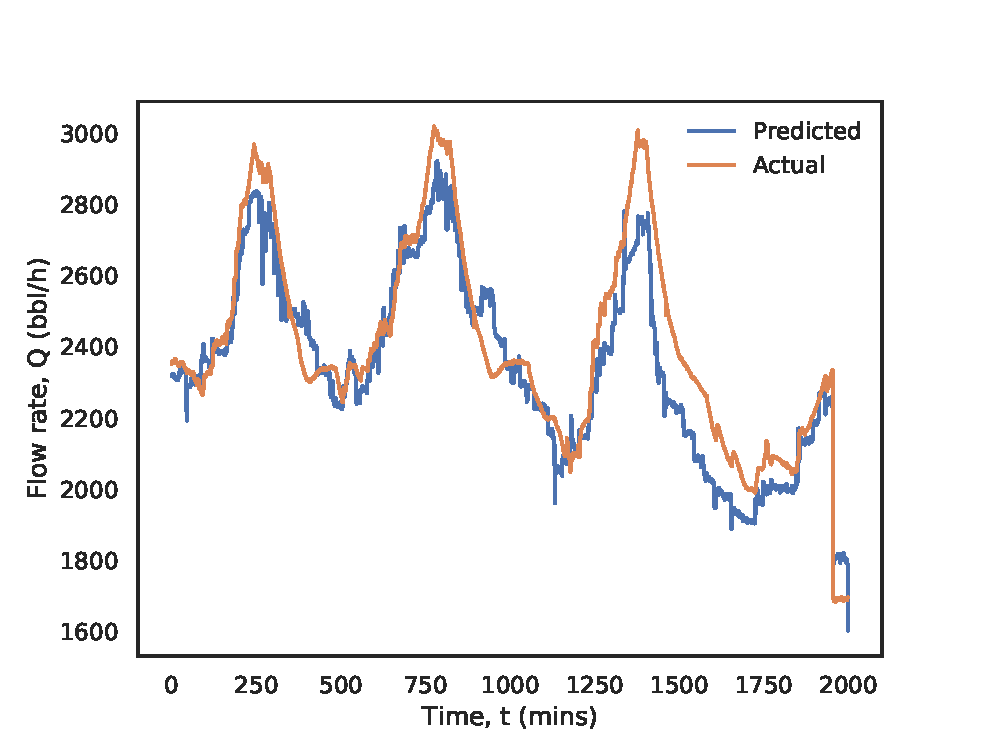
\includegraphics[width=\textwidth]{images/08ls_validation.eps}
         \caption{Predicted vs. actual flow rate for the validation data set.}
         \label{fig:08LSValidation}
     \end{subfigure}
     \hfill
     \begin{subfigure}[b]{0.48\textwidth}
         \centering
         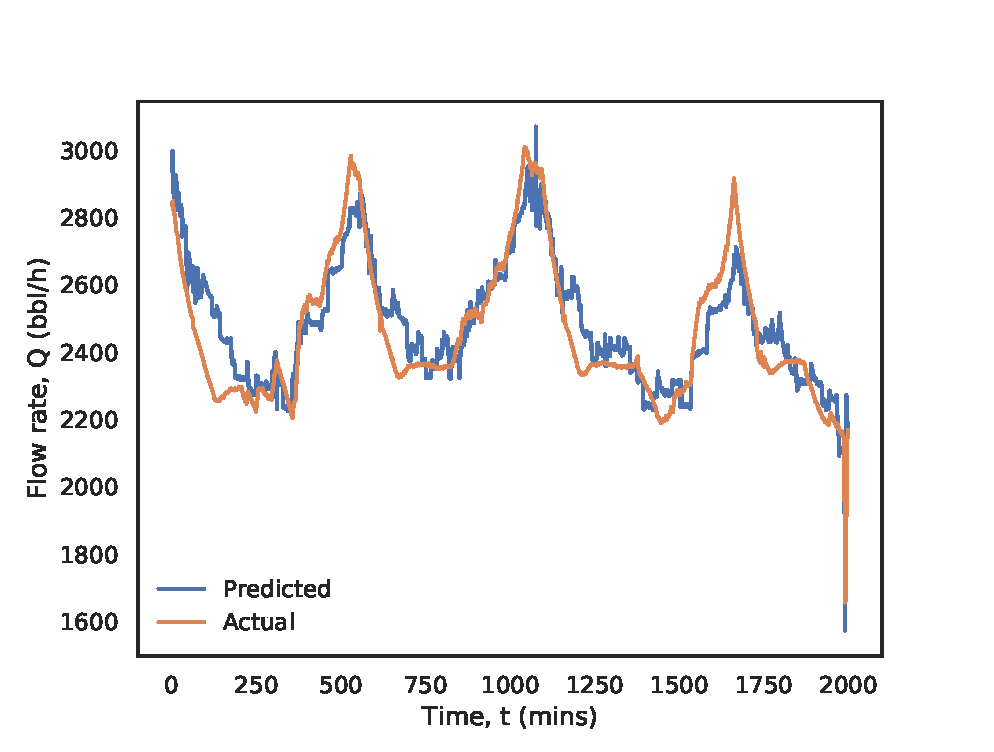
\includegraphics[width=\textwidth]{images/08ls_test.eps}
         \caption{Predicted vs. actual flow rate for the test data set.}
         \label{fig:08LSTest}
     \end{subfigure}
        \caption{Comparison of normal and abnormal density readings.}
        \label{fig:08LSPlots}
\end{figure}
The least squares model is given in Equation \ref{eq:08LS}.  Weights for $x_{11} - x_{14}$ were very small and were omitted.
\begin{multline}
    \hat{y} = 0.10x_1 + 0.15x_2 + 0.13x_3 + 0.04x_4 + 0.04x_5 + 0.09x_6 + 0.12x_7 - 0.01x_8 \\
    + 0.49x_9 + 0.02x_{10} + 0.09x_{11} - 0.18x_{15} + 0.30x_{16} - 0.05x_{17} + 0.04x_{18}
    \label{eq:08LS_eq}
\end{multline}

From Equation \ref{eq:08LS}, it can be seen that turning on the booster pump at Fort Lupton results in a decrease in flow rate.  Theoretically, this is impossible and is most likely caused by noise in the data.  To increase the models ability to reflect reality, engineering knowledge was injected into the model via constraining $x_1 - x_{10}$ to be strictly positive.

%%%%%%%%%%%%%%%%%%%%%%%%%%%%%%%%%%%%%%%%%%%%%%%%%%%%%%%%%%%%%%%%%%%%%
%
% Constrained LS
%
%%%%%%%%%%%%%%%%%%%%%%%%%%%%%%%%%%%%%%%%%%%%%%%%%%%%%%%%%%%%%%%%%%%%%

The new constrained least squares uses the same hyper parameters as shown in Table \ref{tab:08LSHparameters}.  Performance assessment of the constrained least squares is shown in Table \ref{tab:08ConstLSPerformance}.
\begin{table}[h]
    \centering
    {\setstretch{1.5}
    \begin{tabular}{ c | c | c | c}
                             &  Training data    &  Validation data   &    Test data      \\
        \hline
        MAE                  &  98               &    98              &  94     \\
        RMSE                 &  128              &   129              &  123    \\ 
        $R^2$                &  0.91             &   0.91             &  0.74   \\
    \end{tabular}}
    \caption{Performance assessment for the constrained least squares model.}
    \label{tab:08ConstLSPerformance}
\end{table}
The constrained least squares model performance on the validation and test data sets are shown in Figures \ref{fig:08CLSValidation} and \ref{fig:08CLSTest}. The results are nearly identical to the unconstrained model, with lower error in the test data set.
\begin{figure}[h]
     \centering
     \begin{subfigure}[b]{0.48\textwidth}
         \centering
         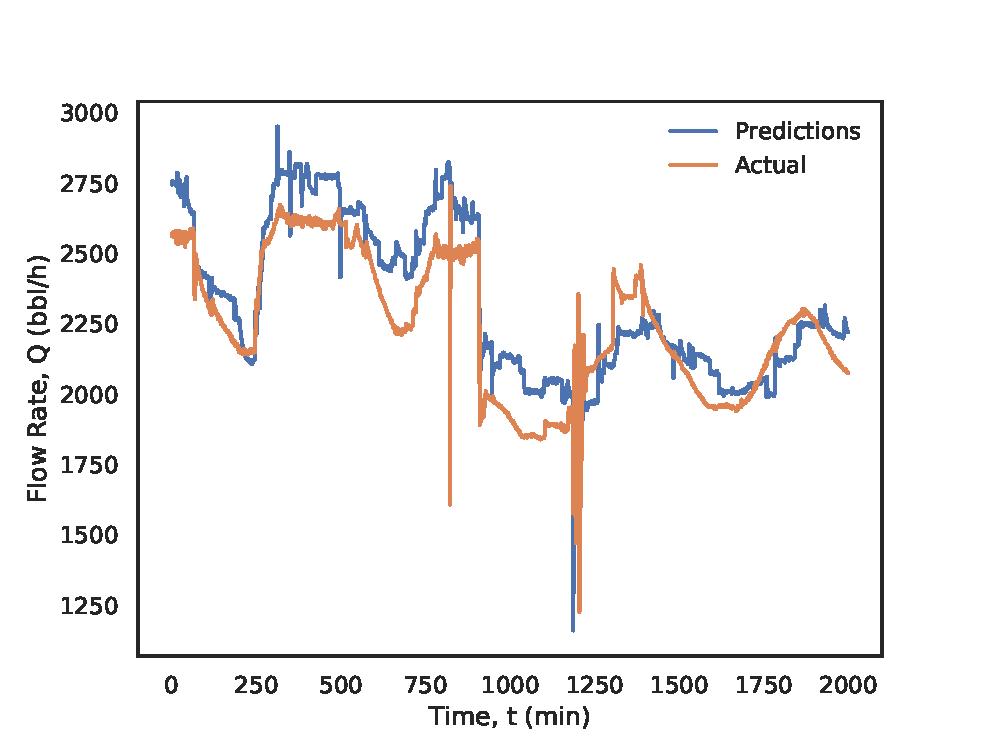
\includegraphics[width=\textwidth]{images/08ConstrainedLS_validation.eps}
         \caption{Predicted vs. actual flow rate for the validation data set.}
         \label{fig:08CLSValidation}
     \end{subfigure}
     \hfill
     \begin{subfigure}[b]{0.48\textwidth}
         \centering
         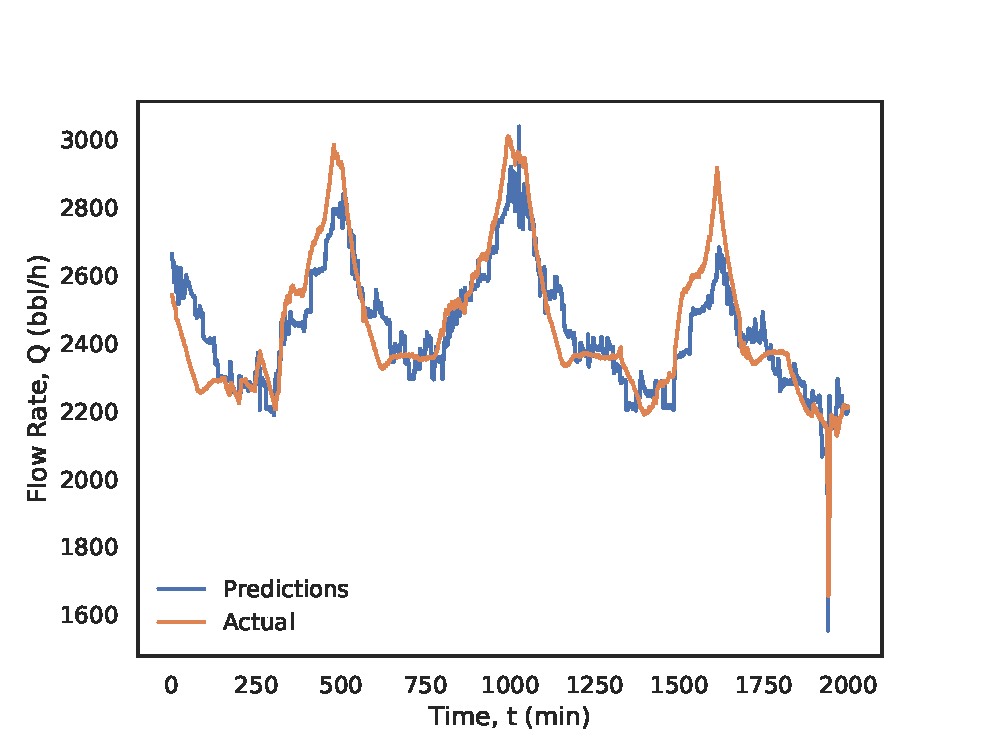
\includegraphics[width=\textwidth]{images/08ConstrainedLS_test.eps}
         \caption{Predicted vs. actual flow rate for the test data set.}
         \label{fig:08CLSTest}
     \end{subfigure}
        \caption{Constrained least squares validation and test plots.}
        \label{fig:08CLSPlots}
\end{figure}

The least squares model is given in Equation \ref{eq:08CLS}.  Weights for $x_{8}, x_{11} - x_{14}$ were very small and were omitted.
\begin{multline}
    \hat{y} = 0.10x_1 + 0.15x_2 + 0.13x_3 + 0.04x_4 + 0.04x_5 + 0.09x_6 + 0.11x_7 \\
    + 0.49x_9 + 0.02x_{10}  - 0.18x_{15} + 0.30x_{16} - 0.05x_{17} + 0.03x_{18}
    \label{eq:08CLS}
\end{multline}

\subsubsection{Non-linear Modelling}
To further increase the accuracy of the models, the following non-linear methods were explored for modelling the pipeline flow rate:
\begin{itemize}
    \item Polynomial models
    \begin{itemize}
        \item Quadratic model
        \item Square-root model
    \end{itemize}
    \item Feed-forward neural networks
    \begin{itemize}
        \item Small neural network (3 layers, 20 nodes per layer)
        \item Medium neural network (6 layers, 30 nodes per layer)
        \item Large neural network (8 layers, 40 nodes per layer)
    \end{itemize}
    \item Linear parameter-varying model
\end{itemize}

%%%%%%%%%%%%%%%%%%%%%%%%%%%%%%%%%%%%%%%%%%%%%%%%%%%%%%%%%%%%%%%%%%%%%
%
%  Quadratic and Sqrt models
%
%%%%%%%%%%%%%%%%%%%%%%%%%%%%%%%%%%%%%%%%%%%%%%%%%%%%%%%%%%%%%%%%%%%%%

The quadratic and square-root model structures given by Equations \ref{eq:08quad_model} and \ref{eq:08sqrt_model}, respectively:
\begin{equation}
    \hat{y} = W_1^T X^2 + W^T_2 X + b
    \label{eq:08quad_model}
\end{equation}
\begin{equation}
    \hat{y} = W_1^T X^{1/2} + W^T_2 X + b
    \label{eq:08sqrt_model}
\end{equation}
where $W_1$ are the weights for the squared and square rooted variables for the quadratic and square-root models, respectively. Furthermore, $W_2$ are the weights for the original variables. The hyper parameters for both models are shown in Table \ref{tab:08poly_hp}.
\begin{table}[h]
    \centering
    {\setstretch{1.5}
    \begin{tabular}{ c | c}
        Hyper Parameter                  &  Value       \\
        \hline
        Epochs                           &  1000      \\
        Minibatch size                   &  8192     \\
        Learning rate, $\alpha$          &  0.001    \\
        Regularization, $\lambda$          &  0.001  \\
    \end{tabular}}
    \caption{Hyper parameters for least squares regression.}
    \label{tab:08poly_hp}
\end{table}

The performance assessment of the quadratic and square root models are shown in Table \ref{tab:08quad_sq_performance}. Compared to the constrained least squares, the MAE and RMSE went down by up to 10\% and 9\% when using the polynomial models, respectively.
\begin{table}[h]
    \centering
    {\setstretch{1.5}
    \begin{tabular}{ c | c | c | c}
                             &  Training data     &  Validation data    &    Test data      \\
        \hline
                             &  Quad $\mid$ Sqrt  &   Quad $\mid$ Sqrt  &  Quad $\mid$ Sqrt \\
        \hline
        MAE                  &  92 $\mid$ 89      &    92 $\mid$ 89     &  89 $\mid$ 91   \\
        RMSE                 &  121 $\mid$ 118    &   121 $\mid$ 117    &  120 $\mid$ 115  \\ 
        $R^2$                &  0.92 $\mid$ 0.93  &   0.92 $\mid$ 0.93  &  0.76 $\mid$ 0.81 \\
    \end{tabular}}
    \caption{Performance assessment for the quadratic and square root model.}
    \label{tab:08quad_sq_performance}
\end{table}

The polynomial model performances are shown in Figures \ref{fig:08quad_validation} to \ref{fig:08sqrt_test}.  

\begin{figure}[h]
     \centering
     \begin{subfigure}[b]{0.48\textwidth}
         \centering
         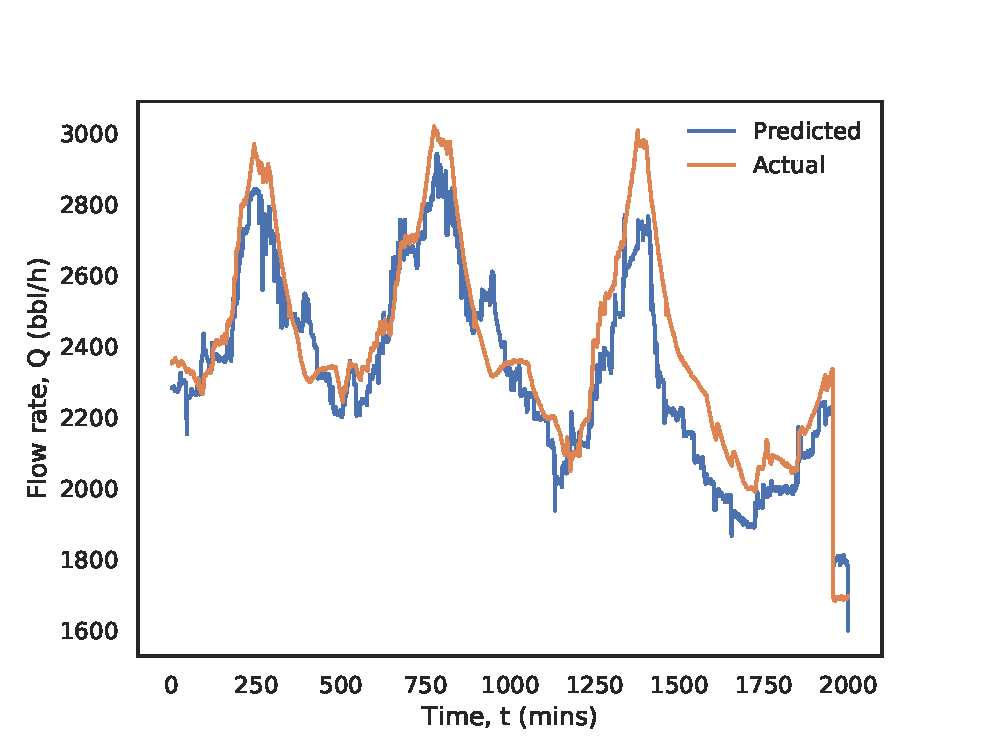
\includegraphics[width=\textwidth]{images/08quad_validation.eps}
         \caption{Predicted vs. actual flow rate for validation data set using the quadratic model.}
         \label{fig:08quad_validation}
     \end{subfigure}
     \hfill
     \begin{subfigure}[b]{0.48\textwidth}
         \centering
         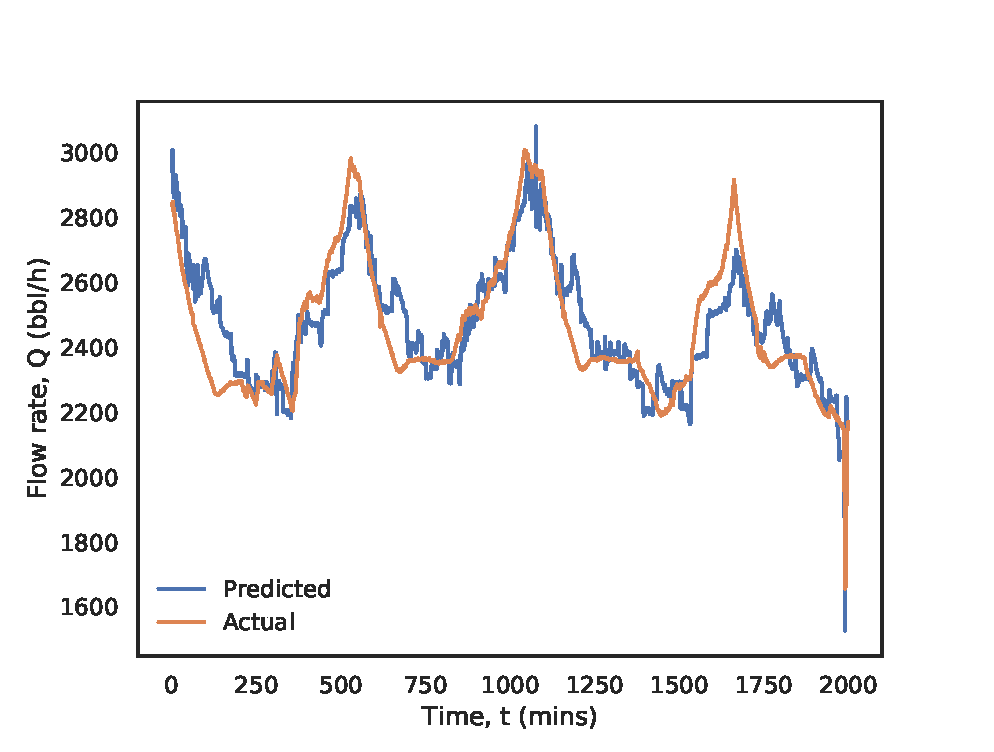
\includegraphics[width=\textwidth]{images/08quad_test.eps}
         \caption{Predicted vs. actual flow rate for the test data set using the quadratic model.}
         \label{fig:08quad_test}
     \end{subfigure}
     \begin{subfigure}[b]{0.48\textwidth}
         \centering
         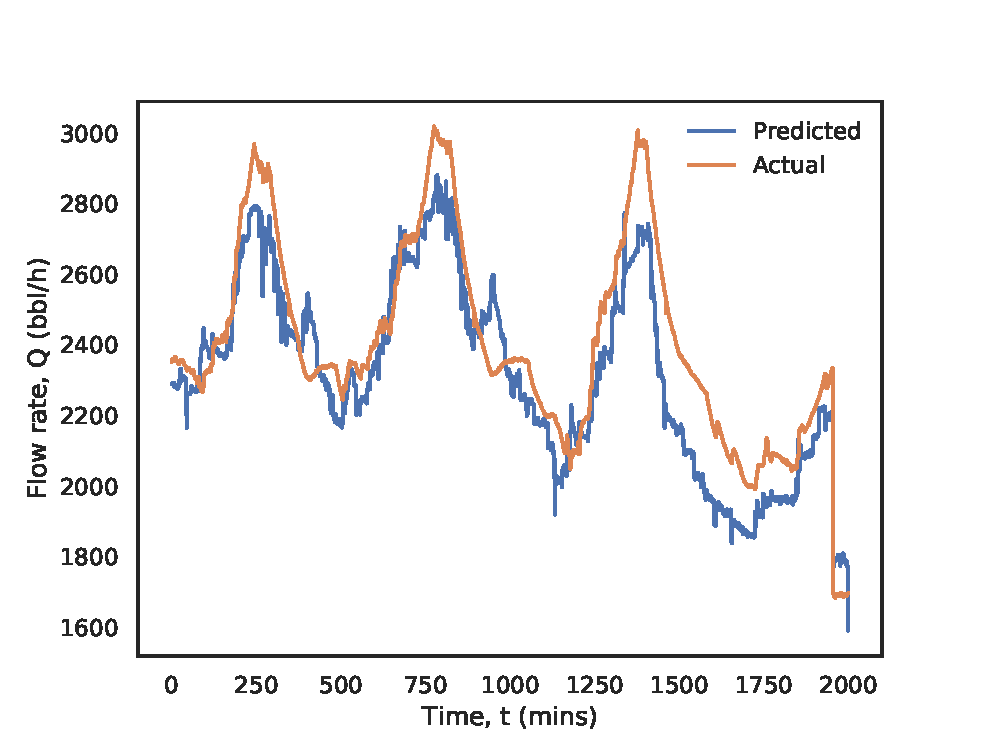
\includegraphics[width=\textwidth]{images/08sqrt_validation.eps}
         \caption{Predicted vs. actual flow rate for the validation data set using the square root model.}
         \label{fig:08sqrt_validation}
     \end{subfigure}
     \hfill
     \begin{subfigure}[b]{0.48\textwidth}
         \centering
         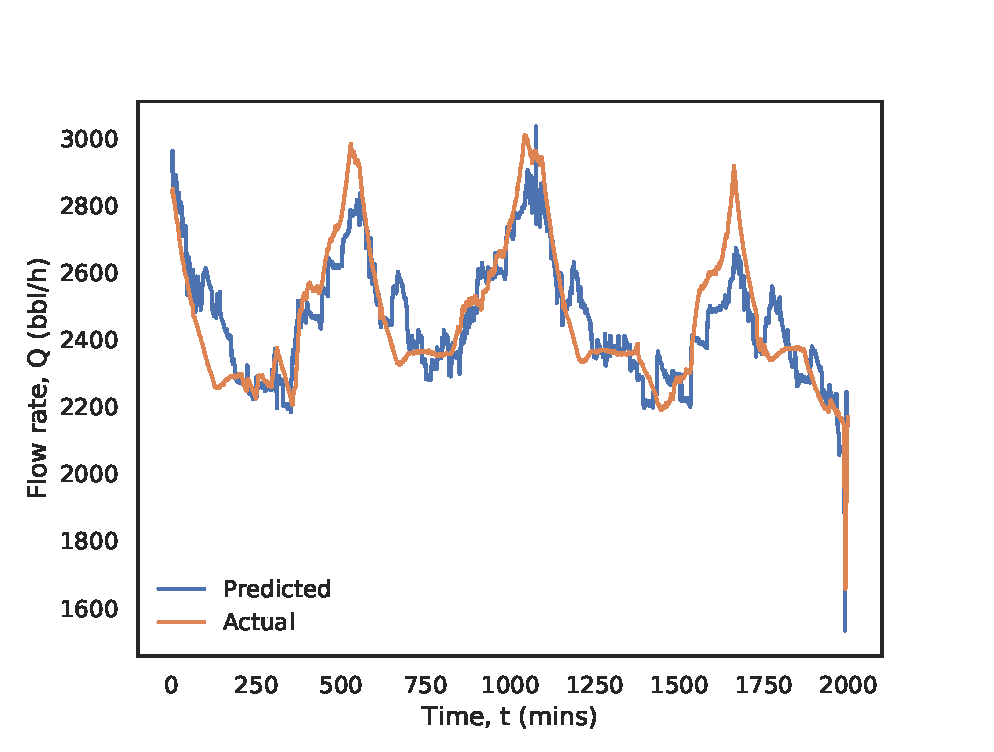
\includegraphics[width=\textwidth]{images/08sqrt_test.eps}
         \caption{Predicted vs. actual flow rate for the test data set using the square root model.}
         \label{fig:08sqrt_test}
     \end{subfigure}
        \caption{Polynomial regression validation and test plots.}
        \label{fig:08PolynomialPlots}
\end{figure}

%%%%%%%%%%%%%%%%%%%%%%%%%%%%%%%%%%%%%%%%%%%%%%%%%%%%%%%%%%%%%%%%%%%%%
%
% Neural Network Models
%
%%%%%%%%%%%%%%%%%%%%%%%%%%%%%%%%%%%%%%%%%%%%%%%%%%%%%%%%%%%%%%%%%%%%%

The neural network models

The hyper parameters for each neural network is given in Table \ref{tab:08NN_hp}.
\begin{table}[h]
    \centering
    {\setstretch{1.5}
    \begin{tabular}{ c | c | c | c}
        Hyper Parameter                            &  Small NN  &  Med. NN  & Large NN       \\
        \hline
        Epochs                                     &  700       & 1000      & 1200  \\
        Minibatch size                             &  8192      & 8192      & 8192  \\
        Learning rate, $\alpha$                    &  0.001     & 0.001     & 0.001 \\
        Regularization, $\lambda$                  &  0.001     & 0.001     & 0.001 \\
        Number of layers                           &  3         & 6         & 8     \\
        Neurons per layer                          &  20        & 30        & 40    \\
        Activation function for hidden layers      & ReLU       & ReLU      & ReLU  \\
    \end{tabular}}
    \caption{Hyper parameters for the feed-forward neural network.}
    \label{tab:08NN_hp}
\end{table}

\begin{table}[h]
    \centering
    {\setstretch{1.5}
    \begin{tabular}{ c | c | c | c}
                    &  Training data     &  Validation data    &    Test data      \\
        \hline
                    &  Small $\mid$ Med $\mid$ Large  &   Small $\mid$ Med $\mid$ Large
                    &  Small $\mid$ Med $\mid$ Large \\
        \hline
        MAE         &  48 $\mid$ 42 $\mid$ 38     &    50 $\mid$ 45 $\mid$ 37   
                    &  87 $\mid$ 87 $\mid$ 115   \\
                    
        RMSE        &  66 $\mid$ 58 $\mid$ 57    &   69 $\mid$ 61 $\mid$ 56    
                    &  121 $\mid$ 107 $\mid$ 138 \\ 
                    
        $R^2$       &  0.97 $\mid$ 0.98 $\mid$ 0.99  &   0.91 $\mid$ 0.90 $\mid$ 0.94   
                    &  0.77 $\mid$ 0.83 $\mid$ 0.66 \\
    \end{tabular}}
    \caption{Performance assessment for the quadratic and square root model.}
    \label{tab:08quad_sq_performance}
\end{table}

The performance of the neural networks are shown in Figures \ref{fig:08smallnn_valid} to \ref{fig:08largenn_test}.  

\begin{figure}[h]
     \centering
     \begin{subfigure}[b]{0.48\textwidth}
         \centering
         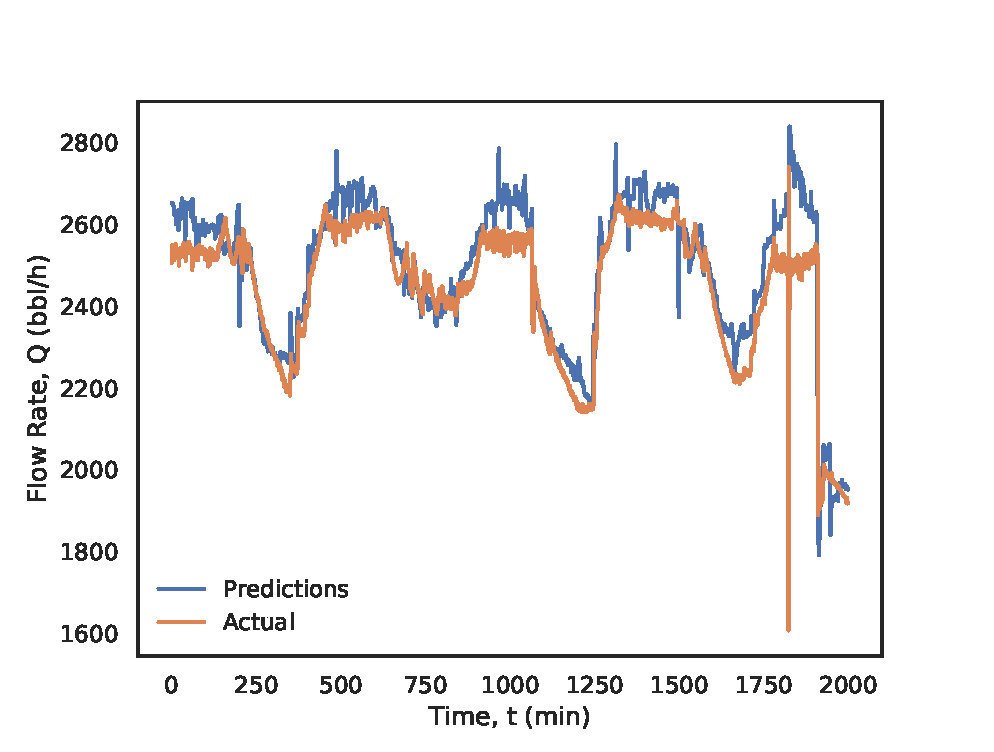
\includegraphics[width=\textwidth]{images/08smallnn_valid.eps}
         \caption{Predicted vs. actual flow rate for validation data set using the small neural net.}
         \label{fig:08smallnn_valid}
     \end{subfigure}
     \hfill
     \begin{subfigure}[b]{0.48\textwidth}
         \centering
         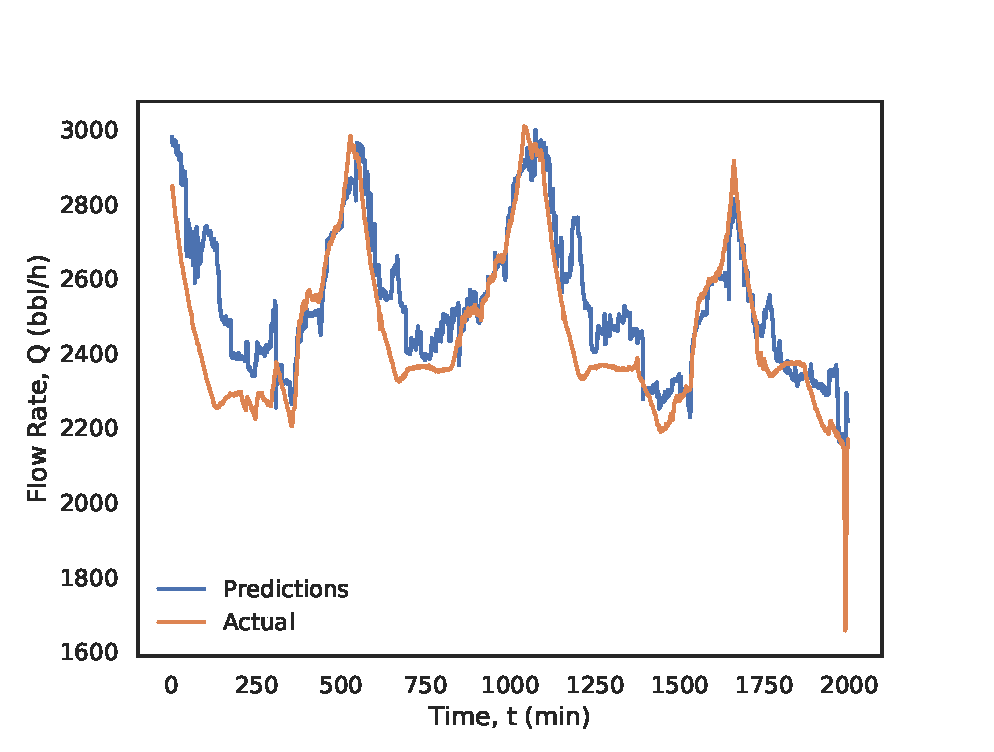
\includegraphics[width=\textwidth]{images/08smallnn_test.eps}
         \caption{Predicted vs. actual flow rate for the test data set using the small neural net.}
         \label{fig:08smallnn_test}
     \end{subfigure}
     \begin{subfigure}[b]{0.48\textwidth}
         \centering
         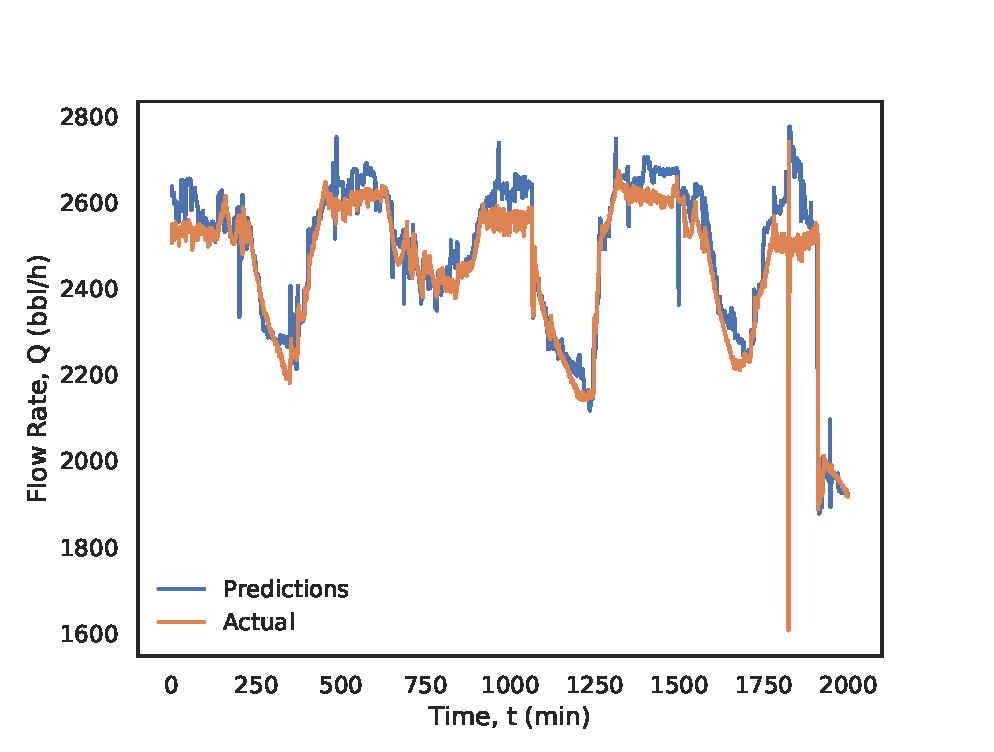
\includegraphics[width=\textwidth]{images/08mednn_valid.eps}
         \caption{Predicted vs. actual flow rate for the validation data set using the medium neural net.}
         \label{fig:08mednn_valid}
     \end{subfigure}
     \hfill
     \begin{subfigure}[b]{0.48\textwidth}
         \centering
         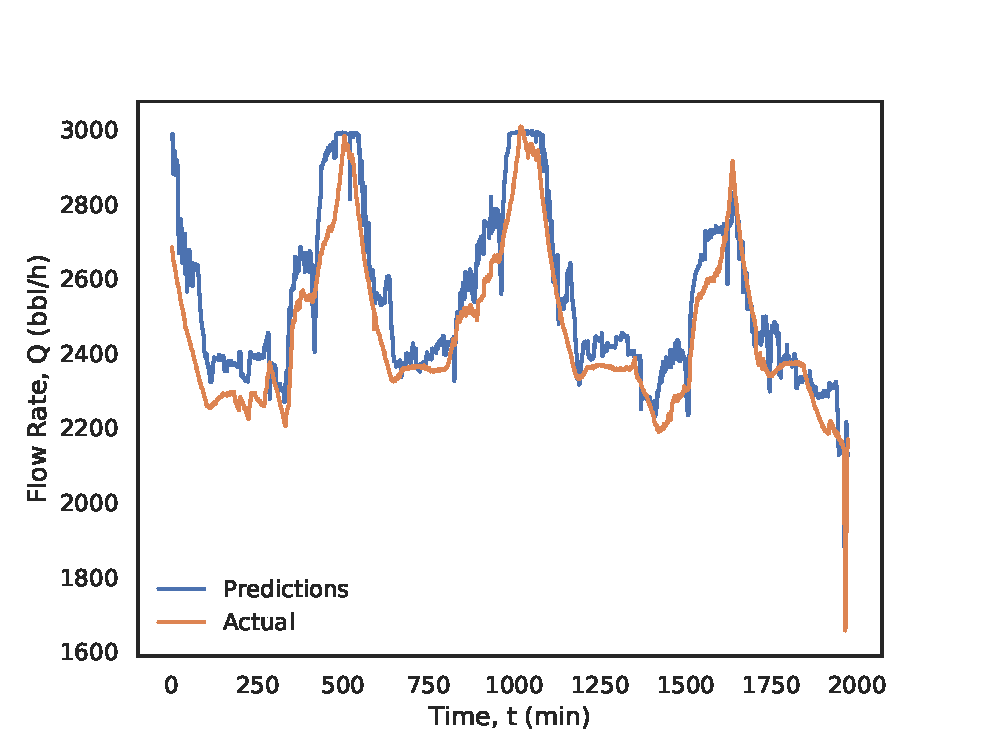
\includegraphics[width=\textwidth]{images/08mednn_test.eps}
         \caption{Predicted vs. actual flow rate for the test data set using the medium neural net.}
         \label{fig:08mednn_test}
     \end{subfigure}
     \begin{subfigure}[b]{0.48\textwidth}
         \centering
         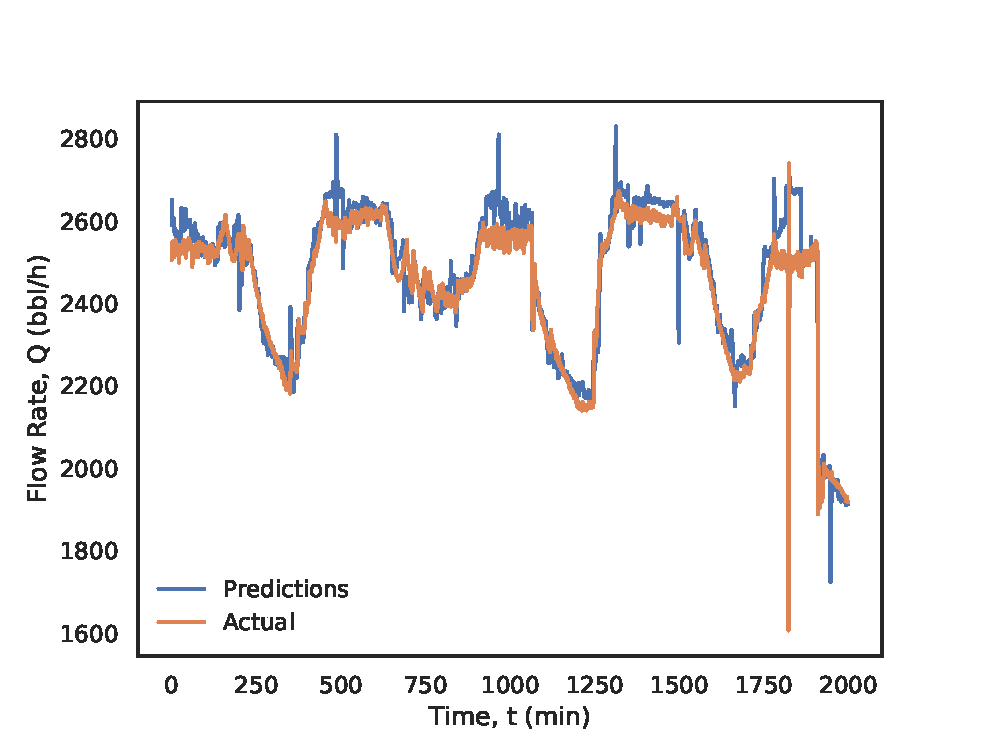
\includegraphics[width=\textwidth]{images/08largenn_valid.eps}
         \caption{Predicted vs. actual flow rate for the validation data set using the large neural net.}
         \label{fig:08largenn_valid}
     \end{subfigure}
     \hfill
     \begin{subfigure}[b]{0.48\textwidth}
         \centering
         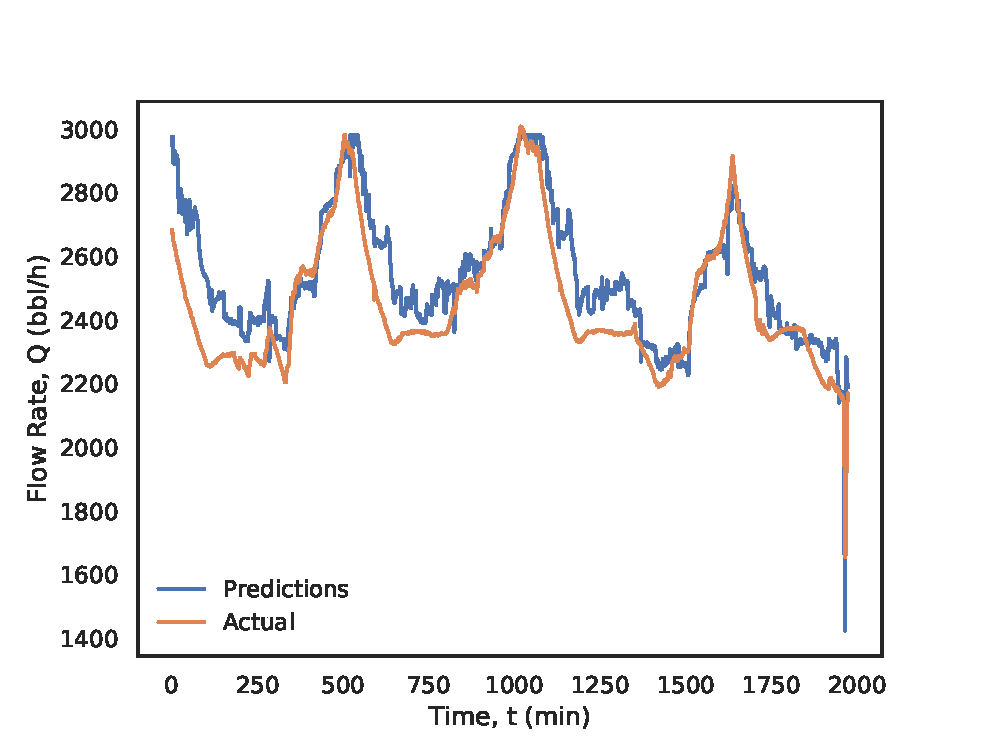
\includegraphics[width=\textwidth]{images/08largenn_test.eps}
         \caption{Predicted vs. actual flow rate for the test data set using the large neural net.}
         \label{fig:08largenn_test}
     \end{subfigure}
        \caption{Feed-forward neural network validation and test plots.}
        \label{fig:08PolynomialPlots}
\end{figure}

%%%%%%%%%%%%%%%%%%%%%%%%%%%%%%%%%%%%%%%%%%%%%%%%%%%%%%%%%%%%%%%%%%%%%
%
% LPV MODELS
%
%%%%%%%%%%%%%%%%%%%%%%%%%%%%%%%%%%%%%%%%%%%%%%%%%%%%%%%%%%%%%%%%%%%%%
Lastly, the linear parameter-varying model (LPV) is given by \cite{LPV}:
\begin{equation}
    \begin{split}
        \hat{y} = W_1^Tx + b_1 \\
        \hat{y} = W_2^Tx + b_2 \\
        ... \\
        \hat{y} = W_n^Tx + b_n \\
    \end{split}
    \label{eq:08LPV_structure}
\end{equation}
where $n \geq 1$ represents the number of linear models used to capture the data set. Here, $W_n$ and $b_n$ are the weights and biases corresponding to the $n^{th}$ model, respectively. 


\subsubsection{Selected Model Structure}
Ultimately, a linear parameter-varying (LPV) model was selected to model this pipeline.  It is clear that the process is heavily non-linear due to the increase in accuracy when switching to a non-linear model structure; therefore, LPV models were selected due to their non-linear nature while still retaining the interpretability of linear models. To enhance credibility, any non-linear model can be approximated by a LPV model via the White's Theorem \cite{LPV}.

\subsubsection{Adaptive Machine Learning}
\paragraph{Online Learning vs. Incremental Learning}
\paragraph{ART: Adaptive Resonance Theory}
\paragraph{Implementation of Adaptive Machine Learning}

\begin{figure}
    \centering
    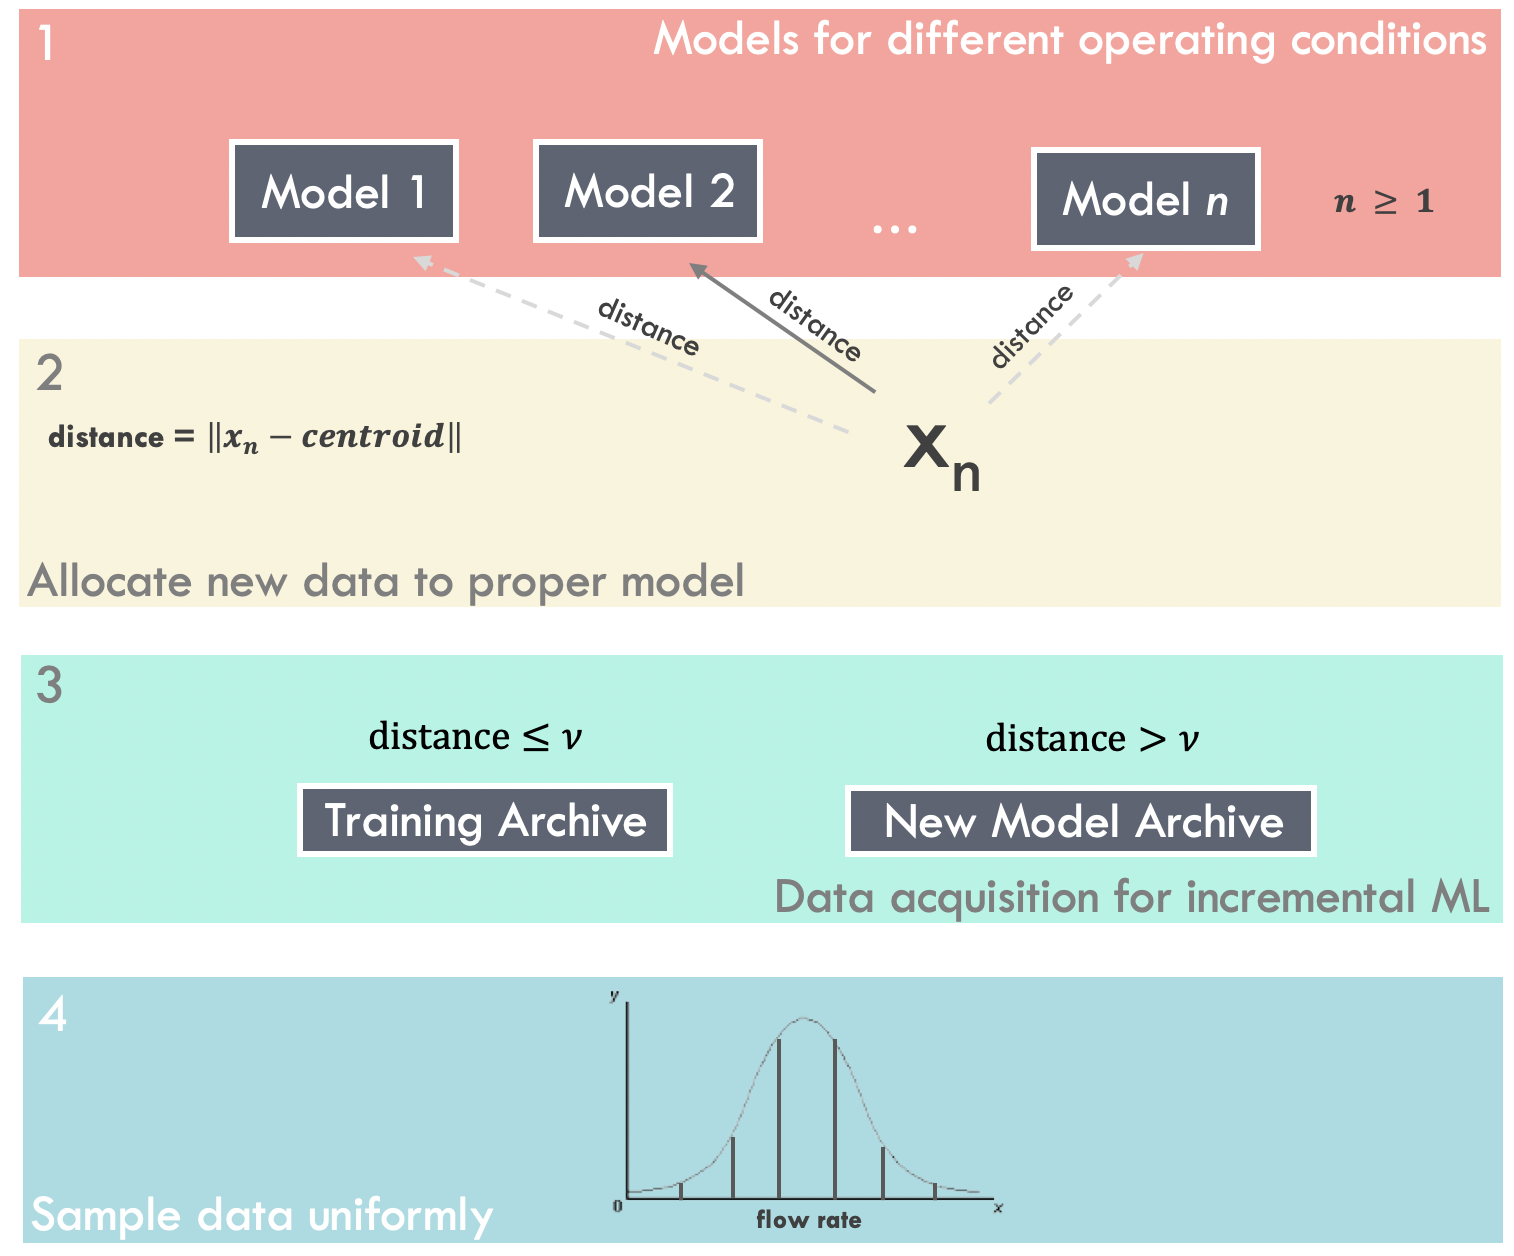
\includegraphics[width=\textwidth]{images/08IncrementalLearning.png}
    \caption{Importance Sampling Incremental Supervised learning architecture.}
    \label{fig:08ART}
\end{figure}

\subsection{Mixed Integer Linear Programming}
\subsection{Conceptual Software Design}
\subsection{Cost Savings and Impact on Society}
